\chapter{Выполнение лабораторной работы}
\label{ch:laba}

В данной главе представлен отчет о разработке Flutter-приложения для синхронизации календаря, аналогичного приложению из ЛР 3, а также анализ его безопасности и взаимодействия с backend-сервисом.

\section{Обзор архитектуры backend-сервиса itmo-calendar}
Backend-сервис \texttt{itmo-calendar} написан на Go и предназначен для предоставления API для работы с расписанием студентов ИТМО и его синхронизации с внешними календарями.

\subsection{API сервиса}
API сервиса определено с использованием Swagger (OpenAPI 2.0). Основные эндпоинты:
\begin{itemize}
    \item \texttt{GET /api/v1/health}: Проверка состояния сервиса.
    \item \texttt{GET /api/v1/\{isu\}/schedule}: Получение расписания пользователя по его номеру ИСУ.
    \item \texttt{GET /api/v1/\{isu\}/ical}: Получение iCalendar (.ics) файла для пользователя.
    \item \texttt{POST /api/v1/subscribe}: Подписка пользователя (регистрация ИСУ и пароля) для генерации и сохранения iCal файла.
\end{itemize}
Аутентификация предполагается через JWT (X-Auth-Token), однако в текущей версии Swagger-спецификации она не форсируется для всех эндпоинтов.

\subsection{Архитектура и внутреннее устройство}
Сервис построен на основе use-case driven архитектуры. Каждый бизнес-сценарий (например, получение расписания, подписка) вынесен в отдельный use case. Это обеспечивает хорошую модульность и тестируемость.
\begin{figure}[h!]
    \centering
    \caption{Общая архитектура backend-сервиса itmo-calendar}
    \label{fig:backend-arch}
    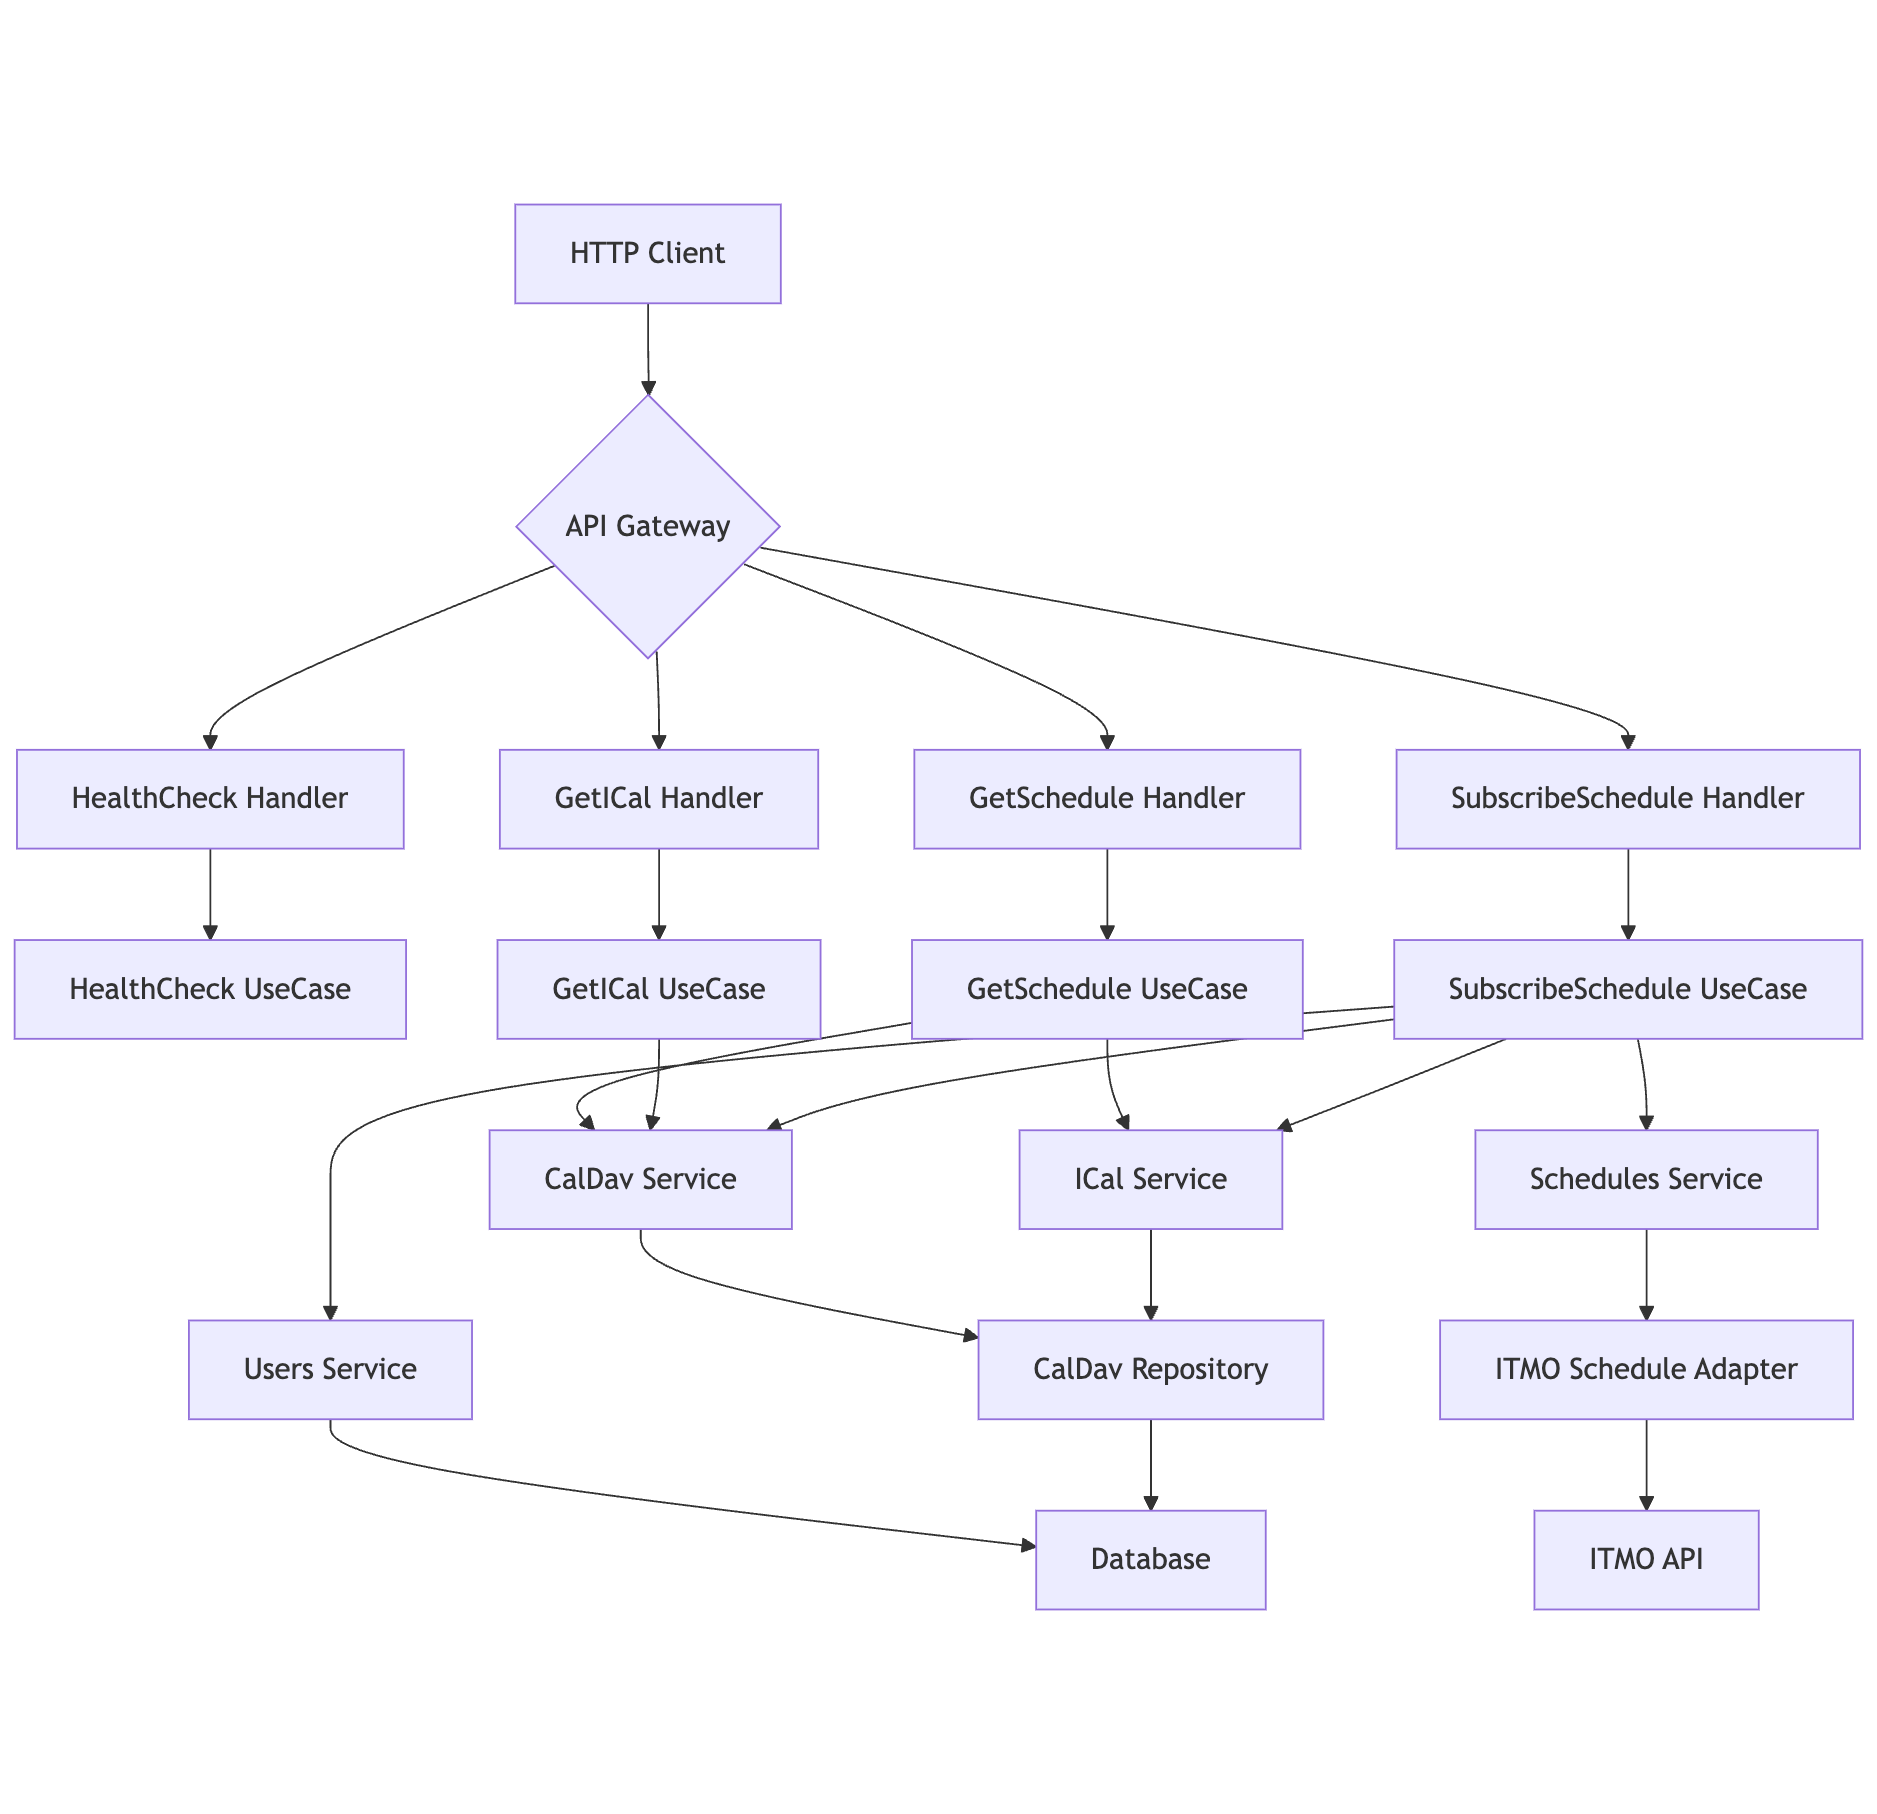
\includegraphics[width=0.6\textwidth]{images/mermaid-1.png}
\end{figure}

\paragraph{Пример Use Case: SubscribeSchedule}
Данный use case отвечает за регистрацию пользователя и создание/обновление его iCalendar файла.
\begin{figure}[h!]
    \centering
    \caption{Диаграмма последовательности для Use Case: SubscribeSchedule}
    \label{fig:subscribe-sequence}
    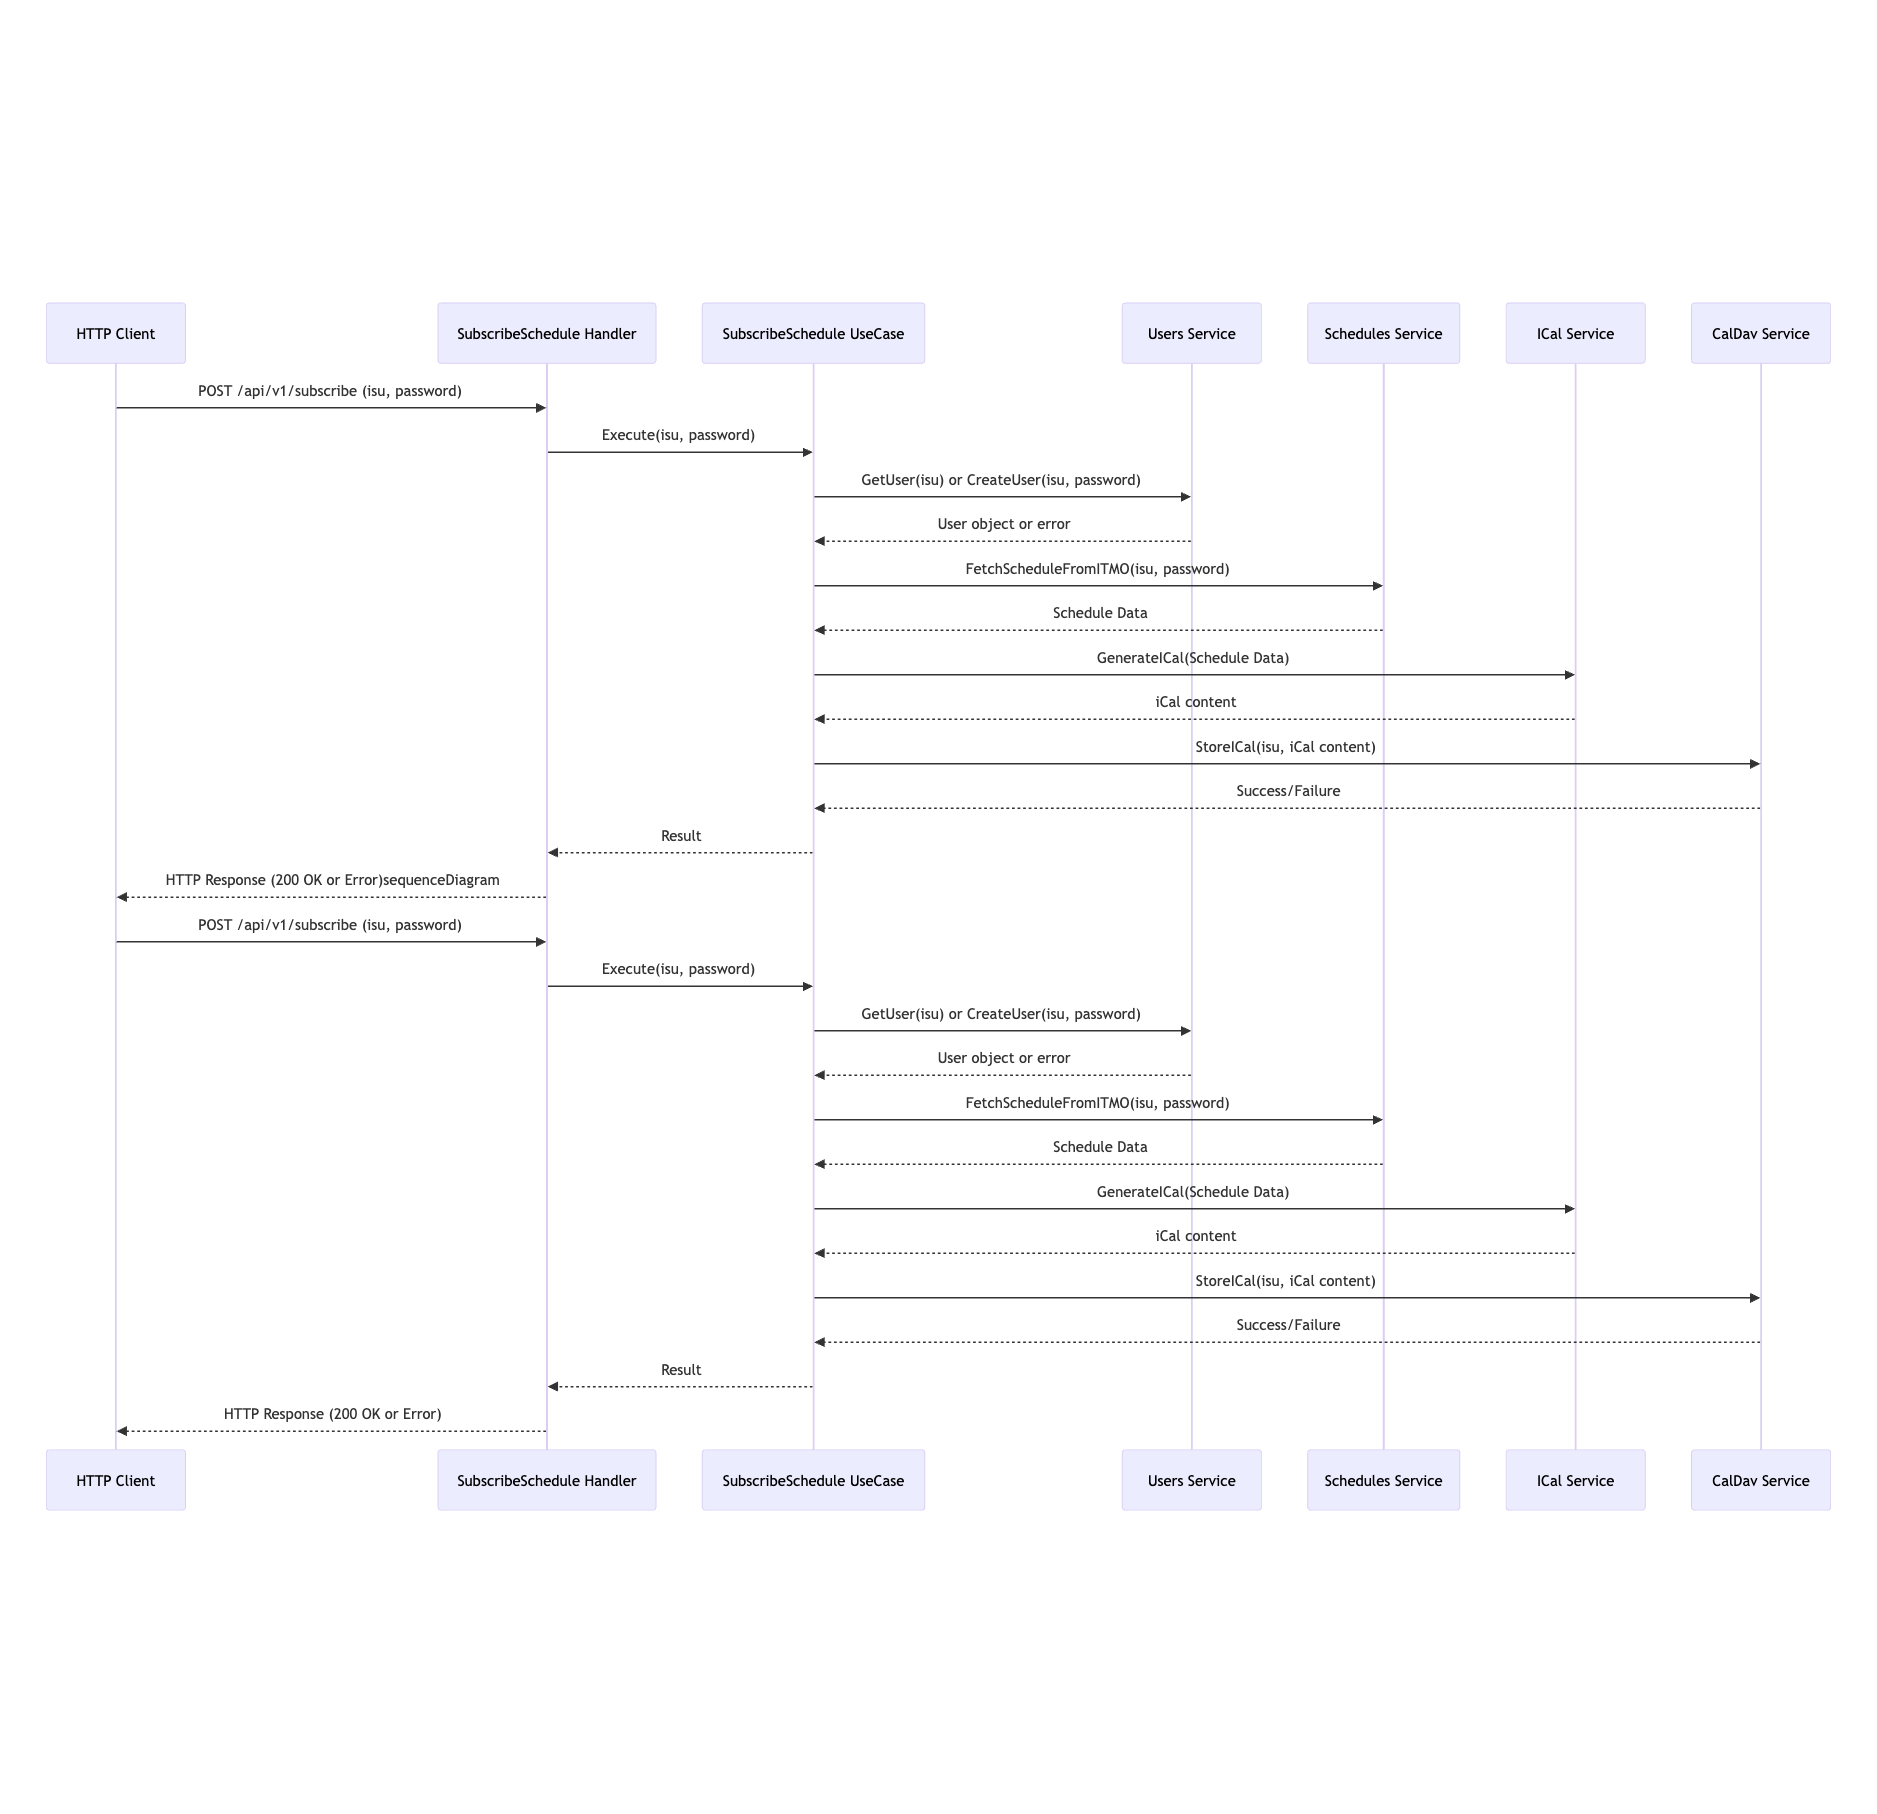
\includegraphics[width=0.6\textwidth]{images/mermaid-2.png}
\end{figure}

\subsection{Аспекты безопасности}
\begin{itemize}
    \item \textbf{Аутентификация}: Планируется использование JWT, что является стандартным подходом для защиты API.
    \item \textbf{Передача данных}: Swagger спецификация указывает на использование HTTPS (подразумевается, т.к. `basePath` не содержит схему, но `consumes` и `produces` `application/json` обычно передаются по HTTPS в production). Локально для разработки используется скрипт \texttt{generate-certs.sh} для создания самоподписанных сертификатов.
    \item \textbf{Обработка ошибок}: Сервис возвращает стандартизированные JSON-ответы об ошибках.
\end{itemize}

\section{Обзор архитектуры Flutter-приложения calendar-sync}
Мобильное приложение \texttt{calendar-sync} разработано на Flutter и предназначено для отображения расписания ИТМО и его синхронизации.

\subsection{Основные компоненты и структура}
Приложение использует следующие ключевые компоненты и подходы:
\begin{itemize}
    \item \textbf{State Management}: Пакет \texttt{provider} для управления состоянием и внедрения зависимостей (\texttt{ApiService}, \texttt{CalendarService}, \texttt{CalendarProvider}).
    \item \textbf{Навигация}: Используется именованная навигация с экранами \texttt{SplashScreen}, \texttt{WelcomeScreen}, \texttt{SyncScreen}.
    \item \textbf{Сервисы}:
    \begin{itemize}
        \item \texttt{ApiService}: Отвечает за все взаимодействия с backend API (запросы на подписку, получение расписания). Включает обработку самоподписанных сертификатов для локальной разработки.
        \item \texttt{CalendarService}: Предположительно, отвечает за взаимодействие с нативными календарями устройства (хотя детали его реализации не были проанализированы в данном отчете).
    \end{itemize}
    \item \textbf{Модели}: \texttt{CalendarEvent} для представления событий расписания.
    \item \textbf{UI}: Стандартные виджеты Flutter, кастомная тема оформления.
\end{itemize}

\begin{figure}[h!]
    \centering
    \caption{Упрощенная схема работы Flutter-приложения calendar-sync}
    \label{fig:flutter-flow}
    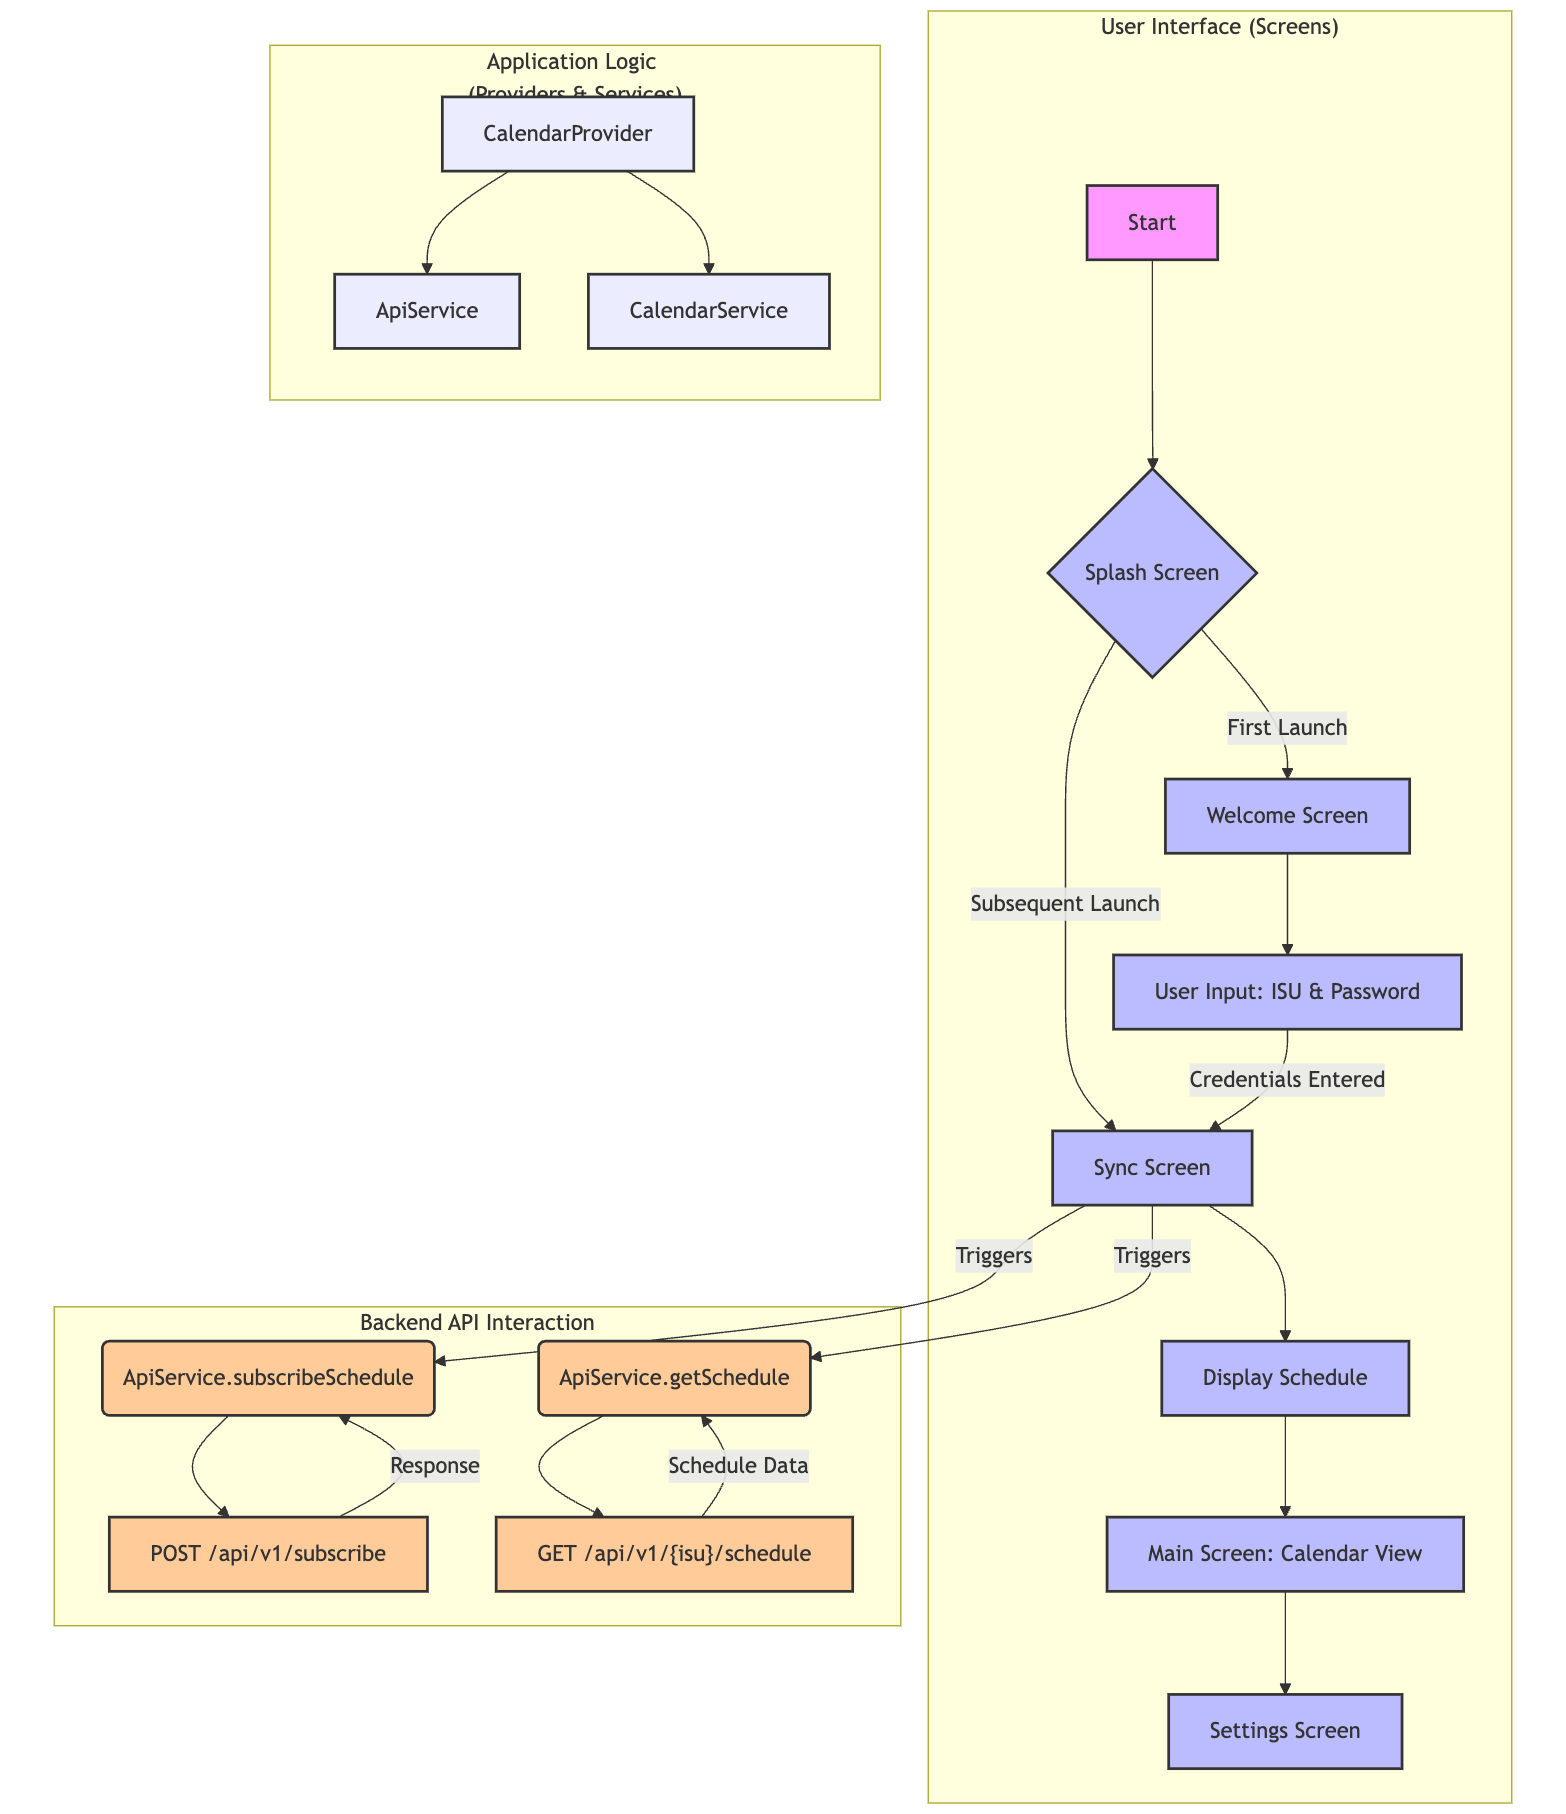
\includegraphics[width=0.6\textwidth]{images/mermaid-3.png}
\end{figure}

\subsection{Реализация запрета на создание скриншотов}
В файле \texttt{lib/main.dart} используется пакет \texttt{screen\_protector} для запрета создания скриншотов. Функция \texttt{\_enableScreenshotBlocking} вызывает \texttt{ScreenProtector.protectDataLeakageWithBlur()} для Android и iOS. Это соответствует требованию лабораторной работы.

\begin{minted}{dart}
Future<void> _enableScreenshotBlocking() async {
  if (defaultTargetPlatform == TargetPlatform.android || 
      defaultTargetPlatform == TargetPlatform.iOS) {
    try {
      await ScreenProtector.protectDataLeakageWithBlur();
    } catch (e) {
      if (kDebugMode) {
        print('Screenshot blocking not supported: $e');
      }
    }
  } else {
    if (kDebugMode) {
      print('Screenshot blocking skipped for desktop');
    }
  }
}
\end{minted}

\subsection{Взаимодействие с backend}
Класс \texttt{ApiService} (\texttt{lib/services/api\_service.dart}) инкапсулирует логику HTTP-запросов к backend. Примечательной особенностью является обработка самоподписанных SSL-сертификатов, что важно для тестирования с локально развернутым backend.
\begin{minted}{dart}
// Фрагмент из ApiService для обработки сертификатов
http.Client _createHttpClient() {
  final httpClient = HttpClient();
  httpClient.badCertificateCallback = 
    (X509Certificate cert, String host, int port) {
    print('Warning: Accepting certificate for $host:$port');
    return true; // Принимаем самоподписанный сертификат
  };
  httpClient.connectionTimeout = const Duration(seconds: 30);
  return IOClient(httpClient);
}
\end{minted}
Это упрощает разработку, но в production-сборке такой подход должен быть заменен на проверку валидных сертификатов.

\section{Анализ APK файлов}
В рамках лабораторной работы были выполнены сборка, декомпиляция и анализ APK-файлов приложения.

\subsection{Получение APK с обфускацией и без}
Были собраны два APK-файла:
\begin{itemize}
    \item \texttt{app-release.apk}: с включенной обфускацией кода (стандартный release-режим Flutter).
    \item \texttt{app-release-no-obfuscate.apk}: предположительно, собран с флагами для минимизации или отключения обфускации (например, \texttt{--no-shrink}).
\end{itemize}
Команды для сборки:
\begin{minted}{bash}
# Сборка с обфускацией (стандартный релиз)
flutter build apk --release

# Сборка без обфускации (или с минимальной)
flutter build apk --release --no-shrink 
# (Примечание: --no-shrink влияет на R8/ProGuard, 
# Dart код обфусцируется самим Flutter)
\end{minted}


\subsection{Декомпиляция APK}
Оба APK-файла были декомпилированы с помощью ApkTool.
\begin{minted}{bash}
apktool d app-release.apk -o report/apks/decompiled-release
apktool d app-release-no-obfuscate.apk -o report/apks/decompiled-no-obfuscate
\end{minted}
Сравнение результатов декомпиляции (файл \texttt{report/apks/diff.txt}) показывает различия, связанные с обфускацией имен классов, методов и полей в smali-коде, а также возможные различия в ресурсах из-за оптимизаций R8.

\textbf{Выдержка из diff-файла (\texttt{report/apks/diff.txt}):}
\begin{small} % Уменьшаем шрифт для содержимого файла
\lstinputlisting[basicstyle=\ttfamily\tiny, breaklines=true, showstringspaces=false]{apks/diff.txt}
\end{small}


\subsection{Сканирование утилитой apkleaks}
Приложение было просканировано утилитой \texttt{apkleaks} для поиска потенциальных утечек чувствительной информации.
\begin{minted}{bash}
apkleaks -f report/apks/app-release.apk -o report/apks/appleaks-result.txt
\end{minted}
Результаты сканирования сохранены в файле \texttt{report/apks/appleaks-result.txt}.

\textbf{Содержимое файла \texttt{report/apks/appleaks-result.txt}:}
\begin{small} % Уменьшаем шрифт для содержимого файла
\lstinputlisting[basicstyle=\ttfamily\tiny, breaklines=true, showstringspaces=false]{apks/appleaks-result.txt}
\end{small}
Как правило, \texttt{apkleaks} может обнаружить URL-адреса, ключи API (если они захардкожены), email и другие строки, которые могут представлять интерес. В данном случае, он мог обнаружить \texttt{https://localhost/api/v1}.

\subsection{Проверка через VirusTotal}
APK-файл \texttt{app-release.apk} был проверен через сервис VirusTotal.
\begin{figure}[h!]
    \centering
    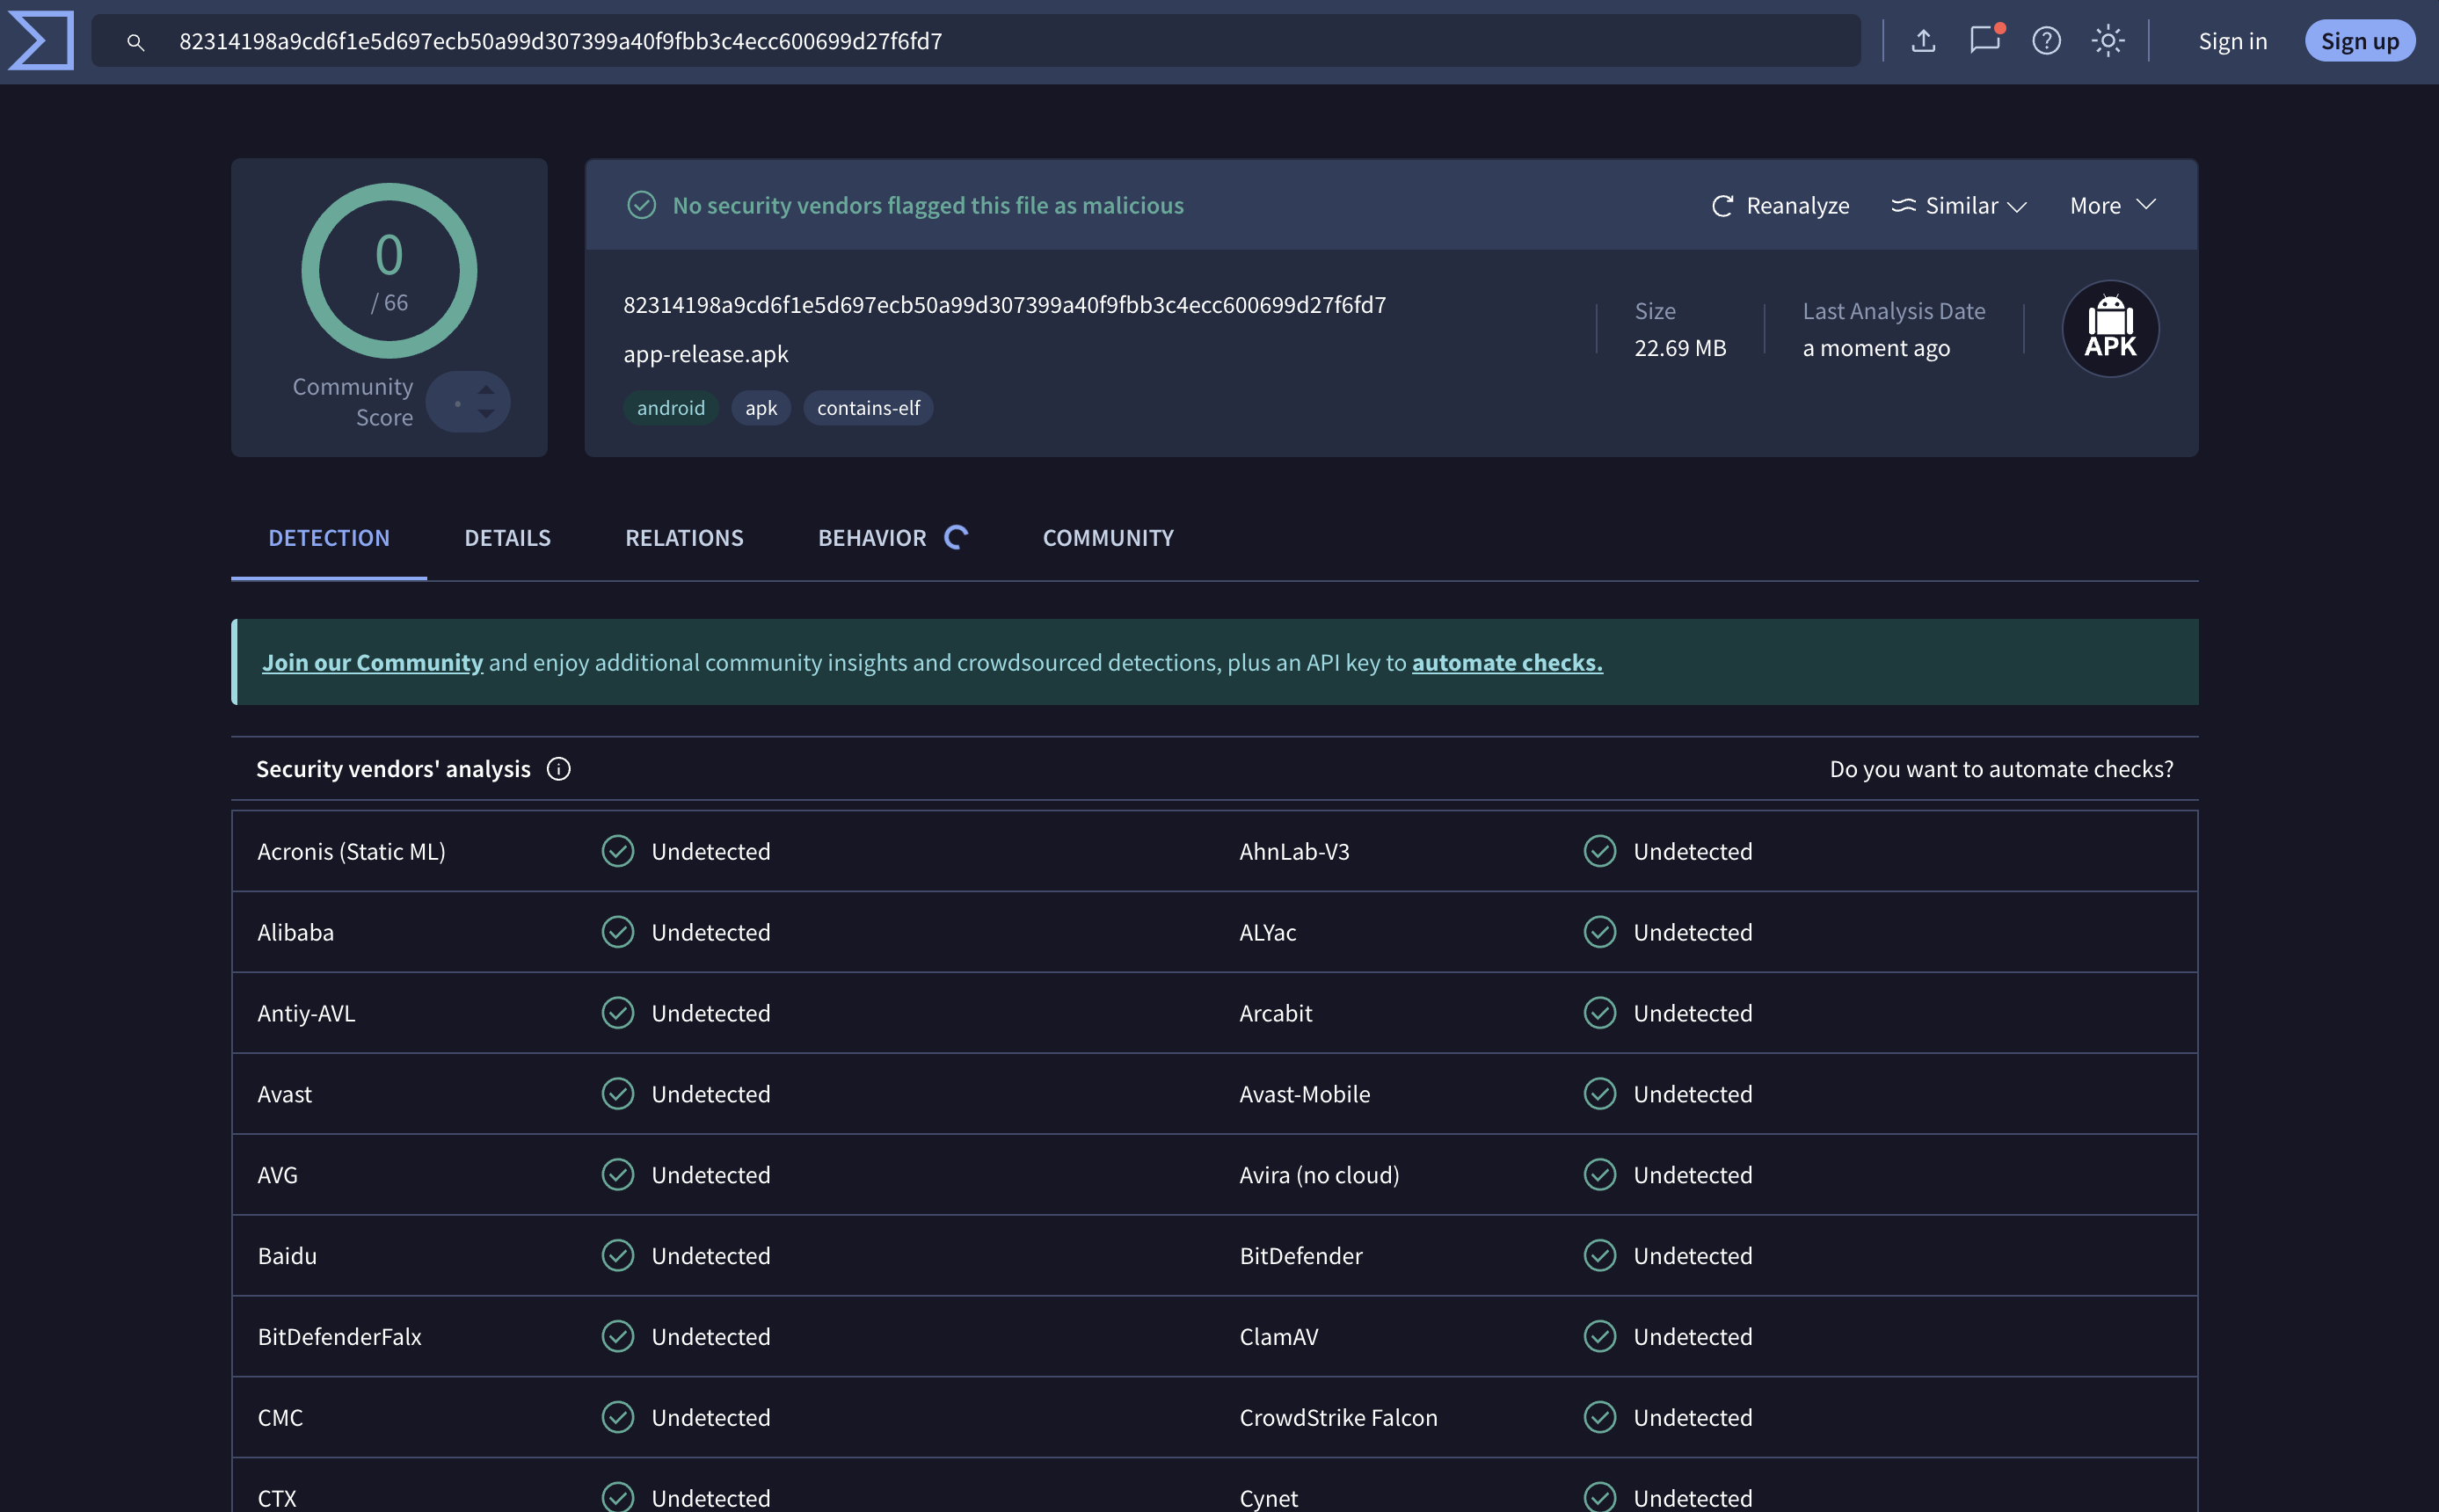
\includegraphics[width=0.9\textwidth]{images/virustotal.png}
    \caption{Результат проверки APK на VirusTotal}
    \label{fig:virustotal}
\end{figure}
Результаты показывают, что большинство антивирусных движков не обнаружили угроз (типично для большинства Flutter-приложений, если не используется специфический вредоносный код).

\section{Скриншоты работы Flutter-приложения}
Далее представлены скриншоты, демонстрирующие работу разработанного Flutter-приложения \texttt{calendar-sync}.

\begin{figure}[h!]
    \centering
    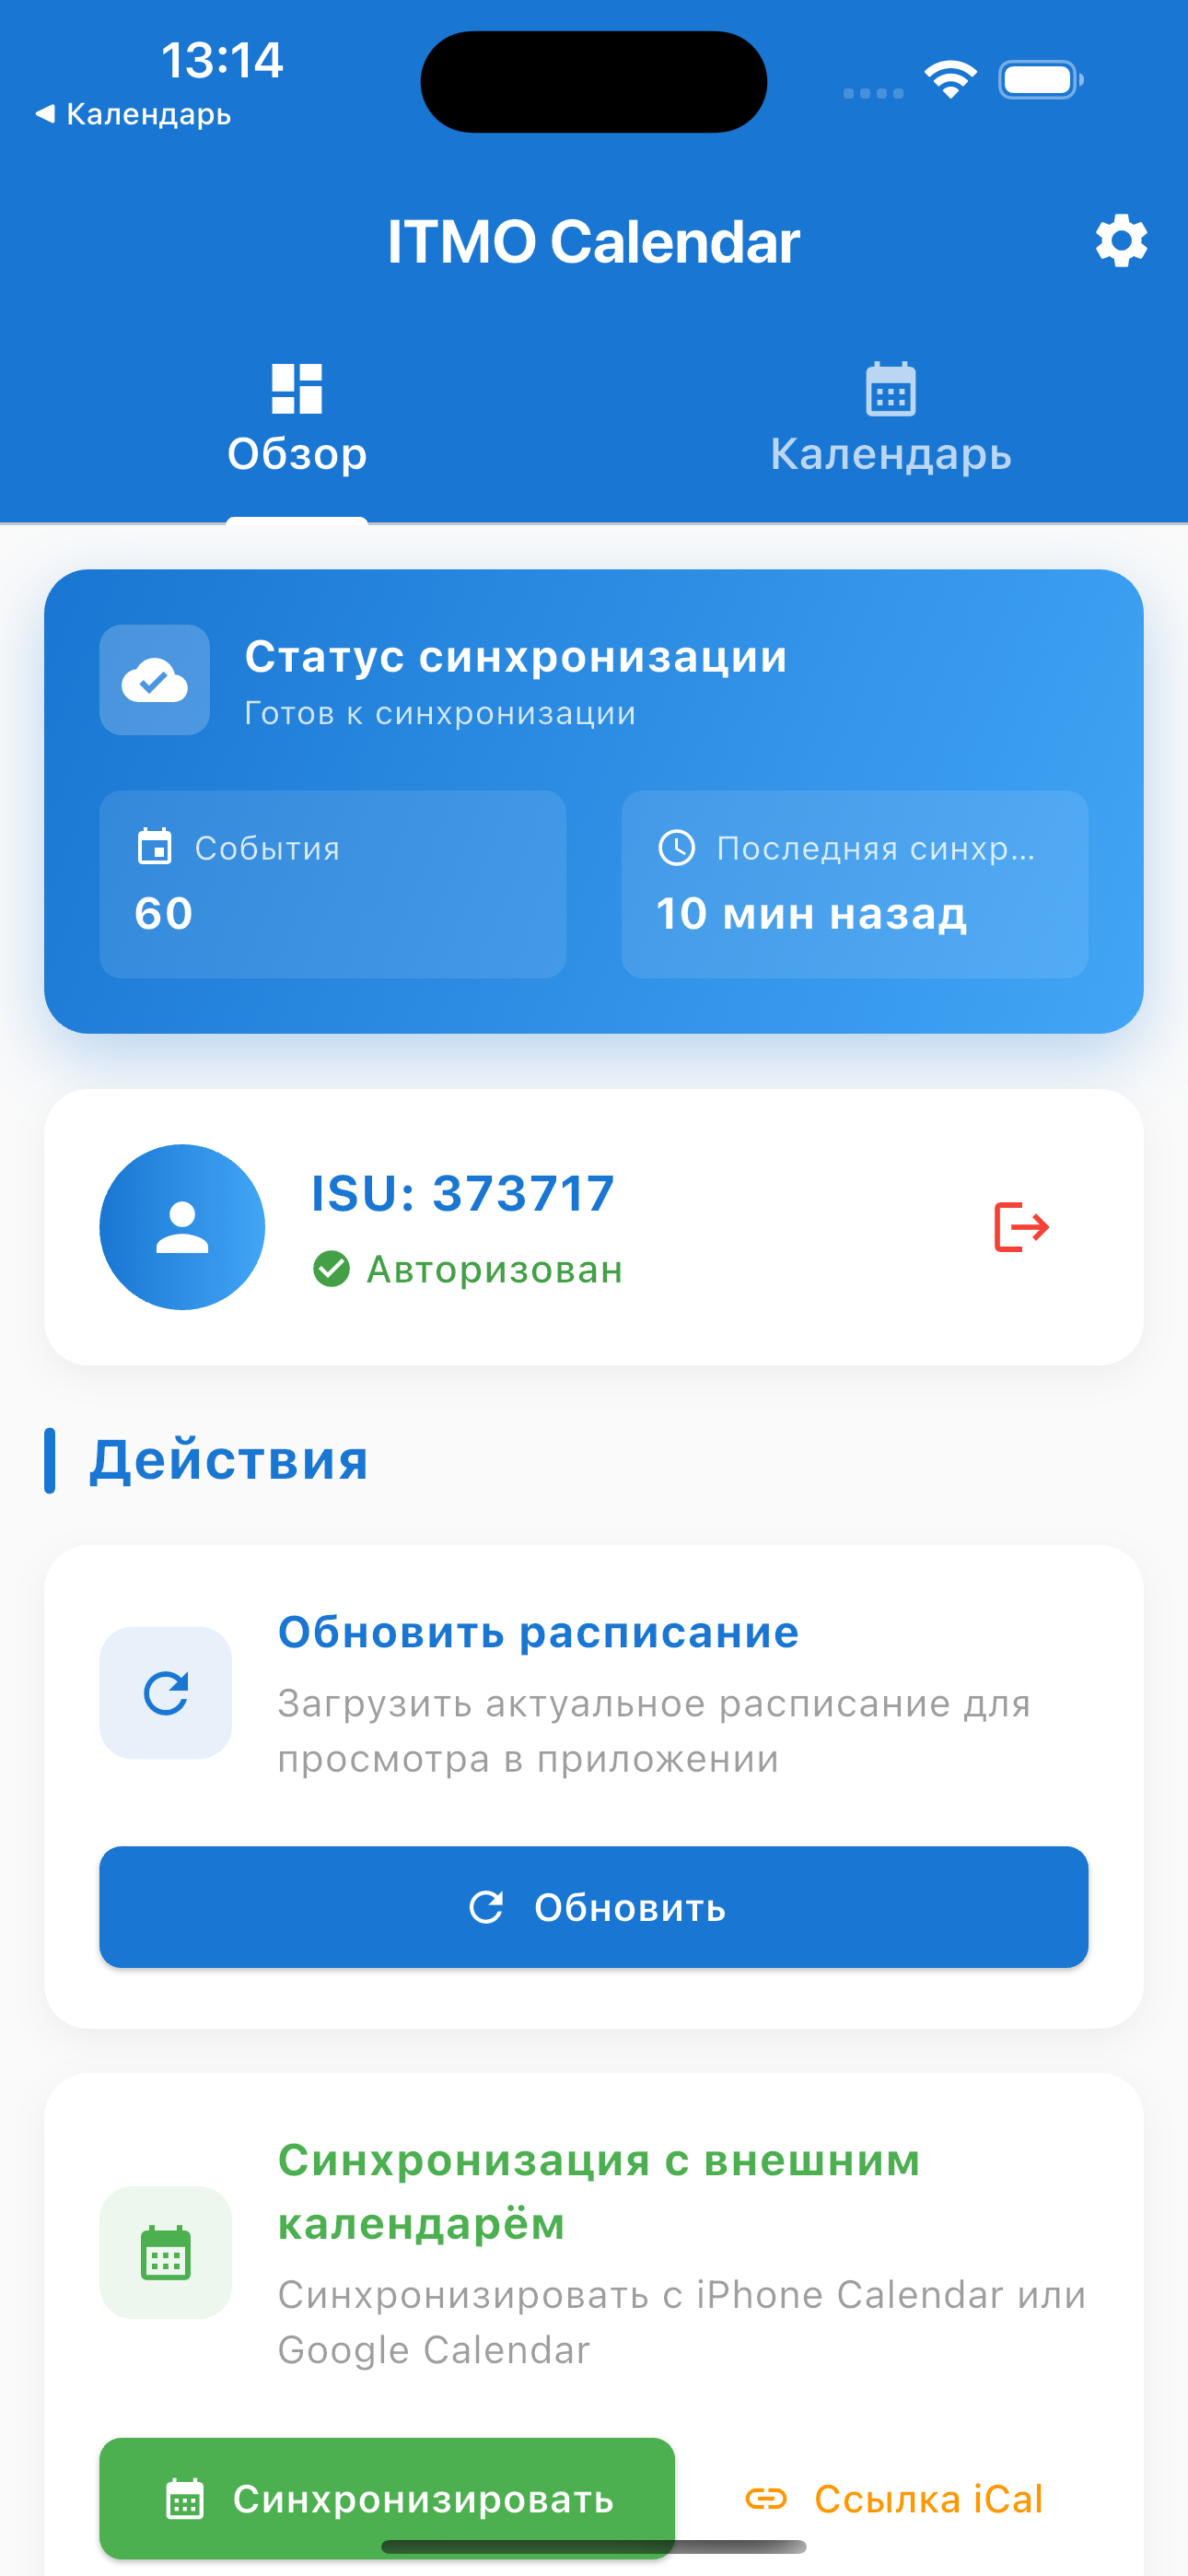
\includegraphics[width=0.6\textwidth]{images/main-screen.png}
    \caption{Главный экран приложения}
    \label{fig:main-screen}
\end{figure}

\begin{figure}[h!]
    \centering
    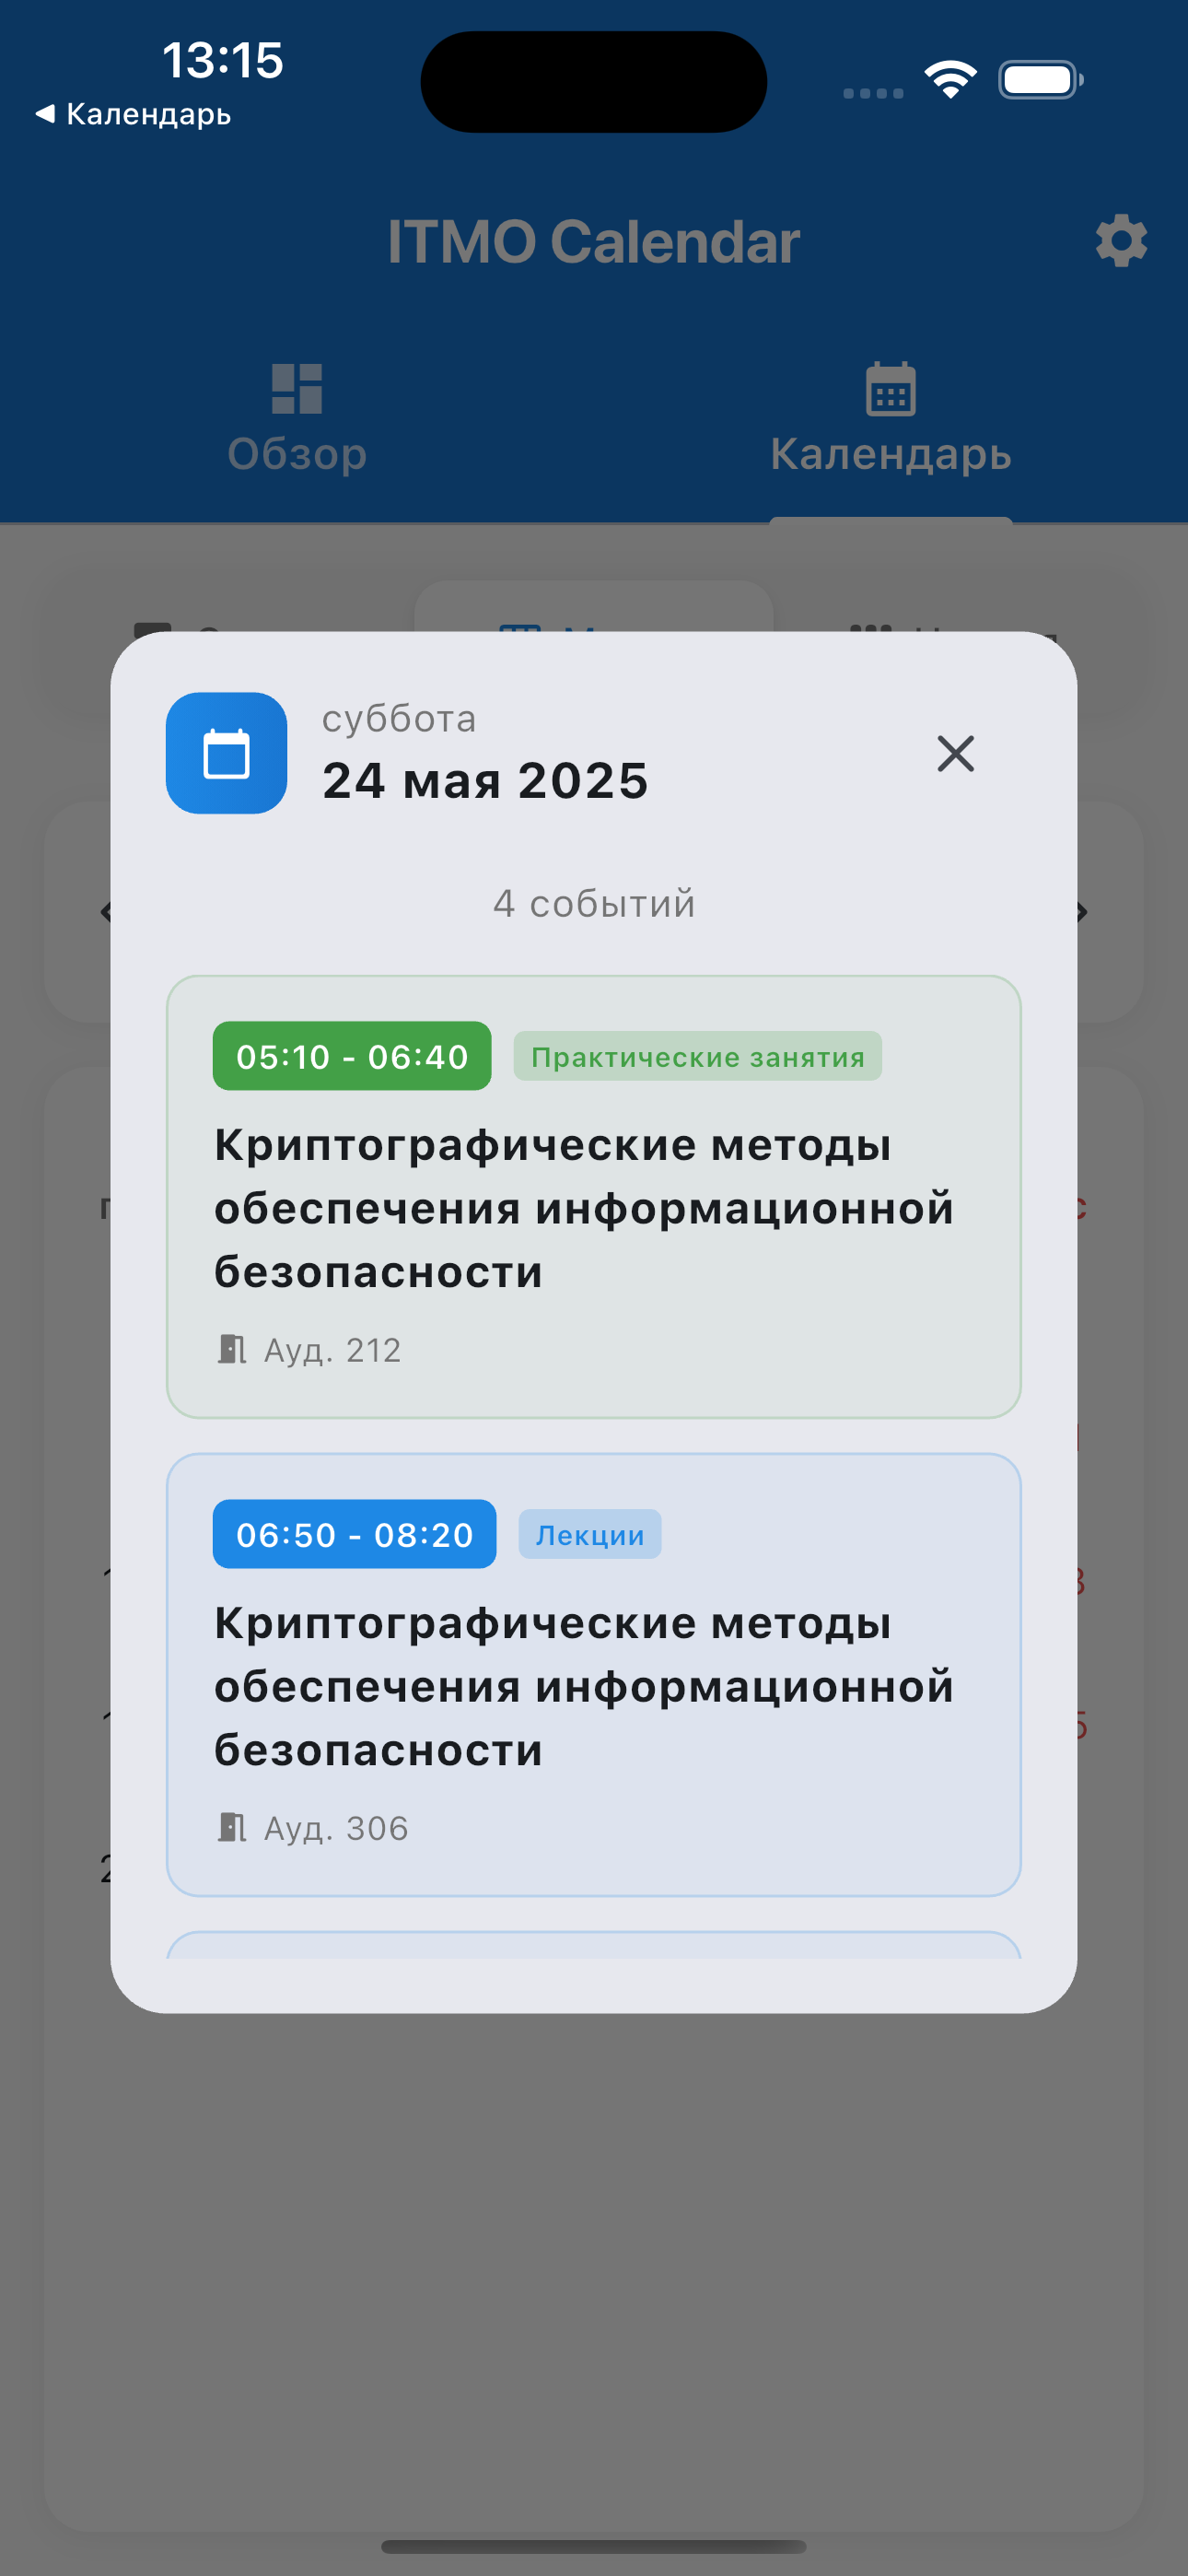
\includegraphics[width=0.6\textwidth]{images/calendar-month.png}
    \caption{Вид календаря на месяц}
    \label{fig:calendar-month}
\end{figure}

\begin{figure}[h!]
    \centering
    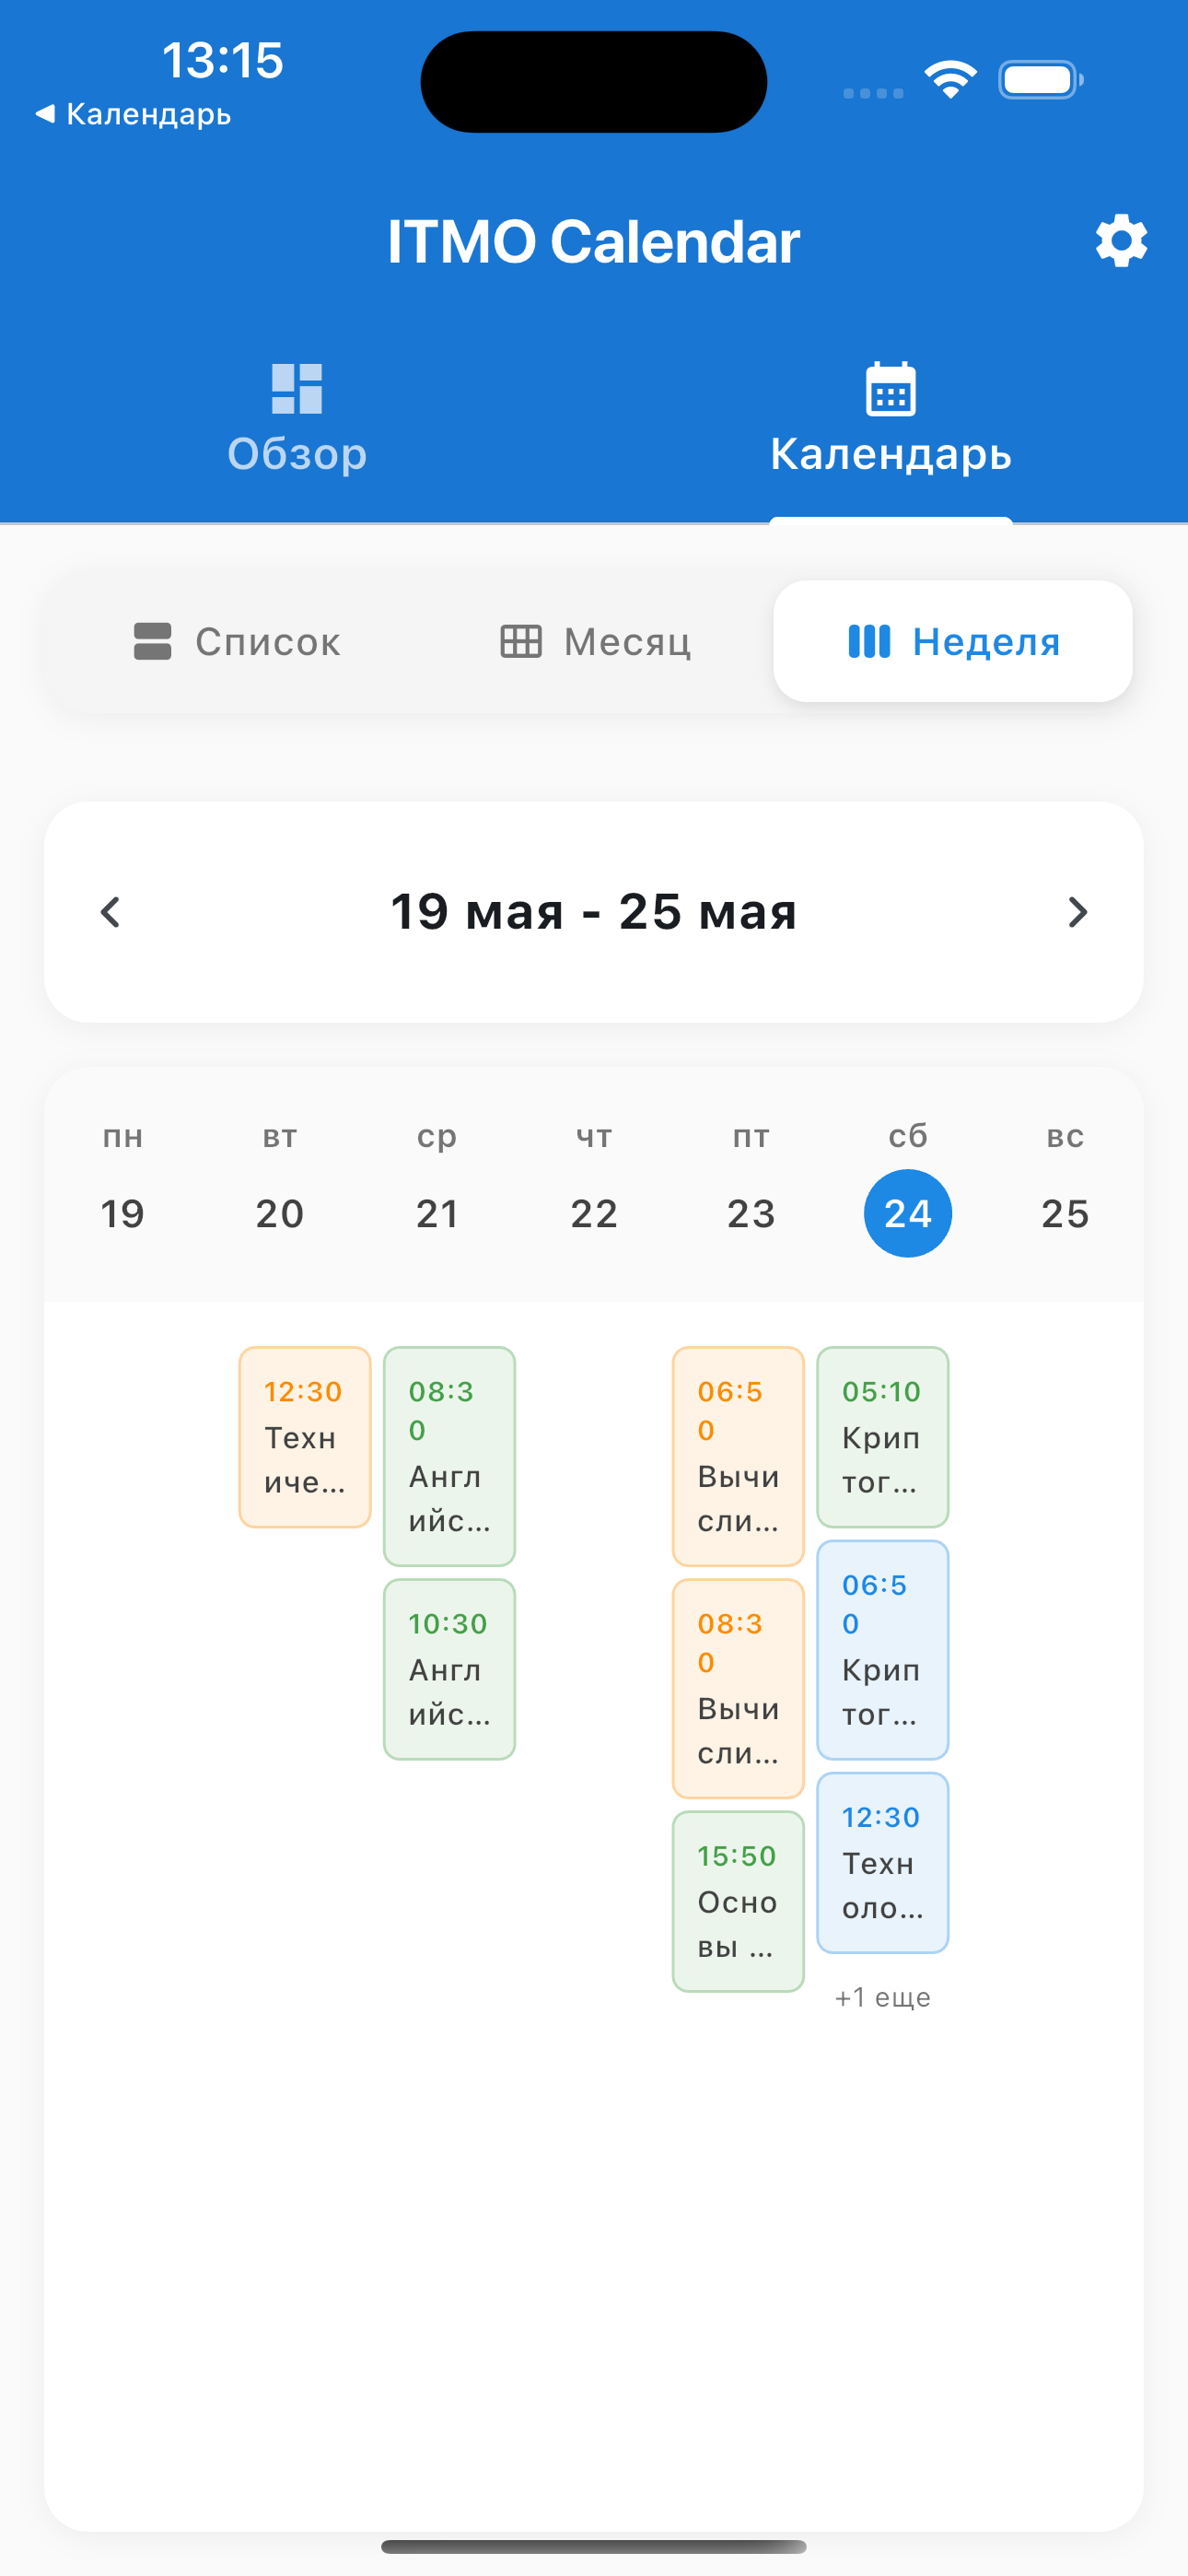
\includegraphics[width=0.6\textwidth]{images/calendar-week.png}
    \caption{Вид календаря на неделю}
    \label{fig:calendar-week}
\end{figure}

\begin{figure}[h!]
    \centering
    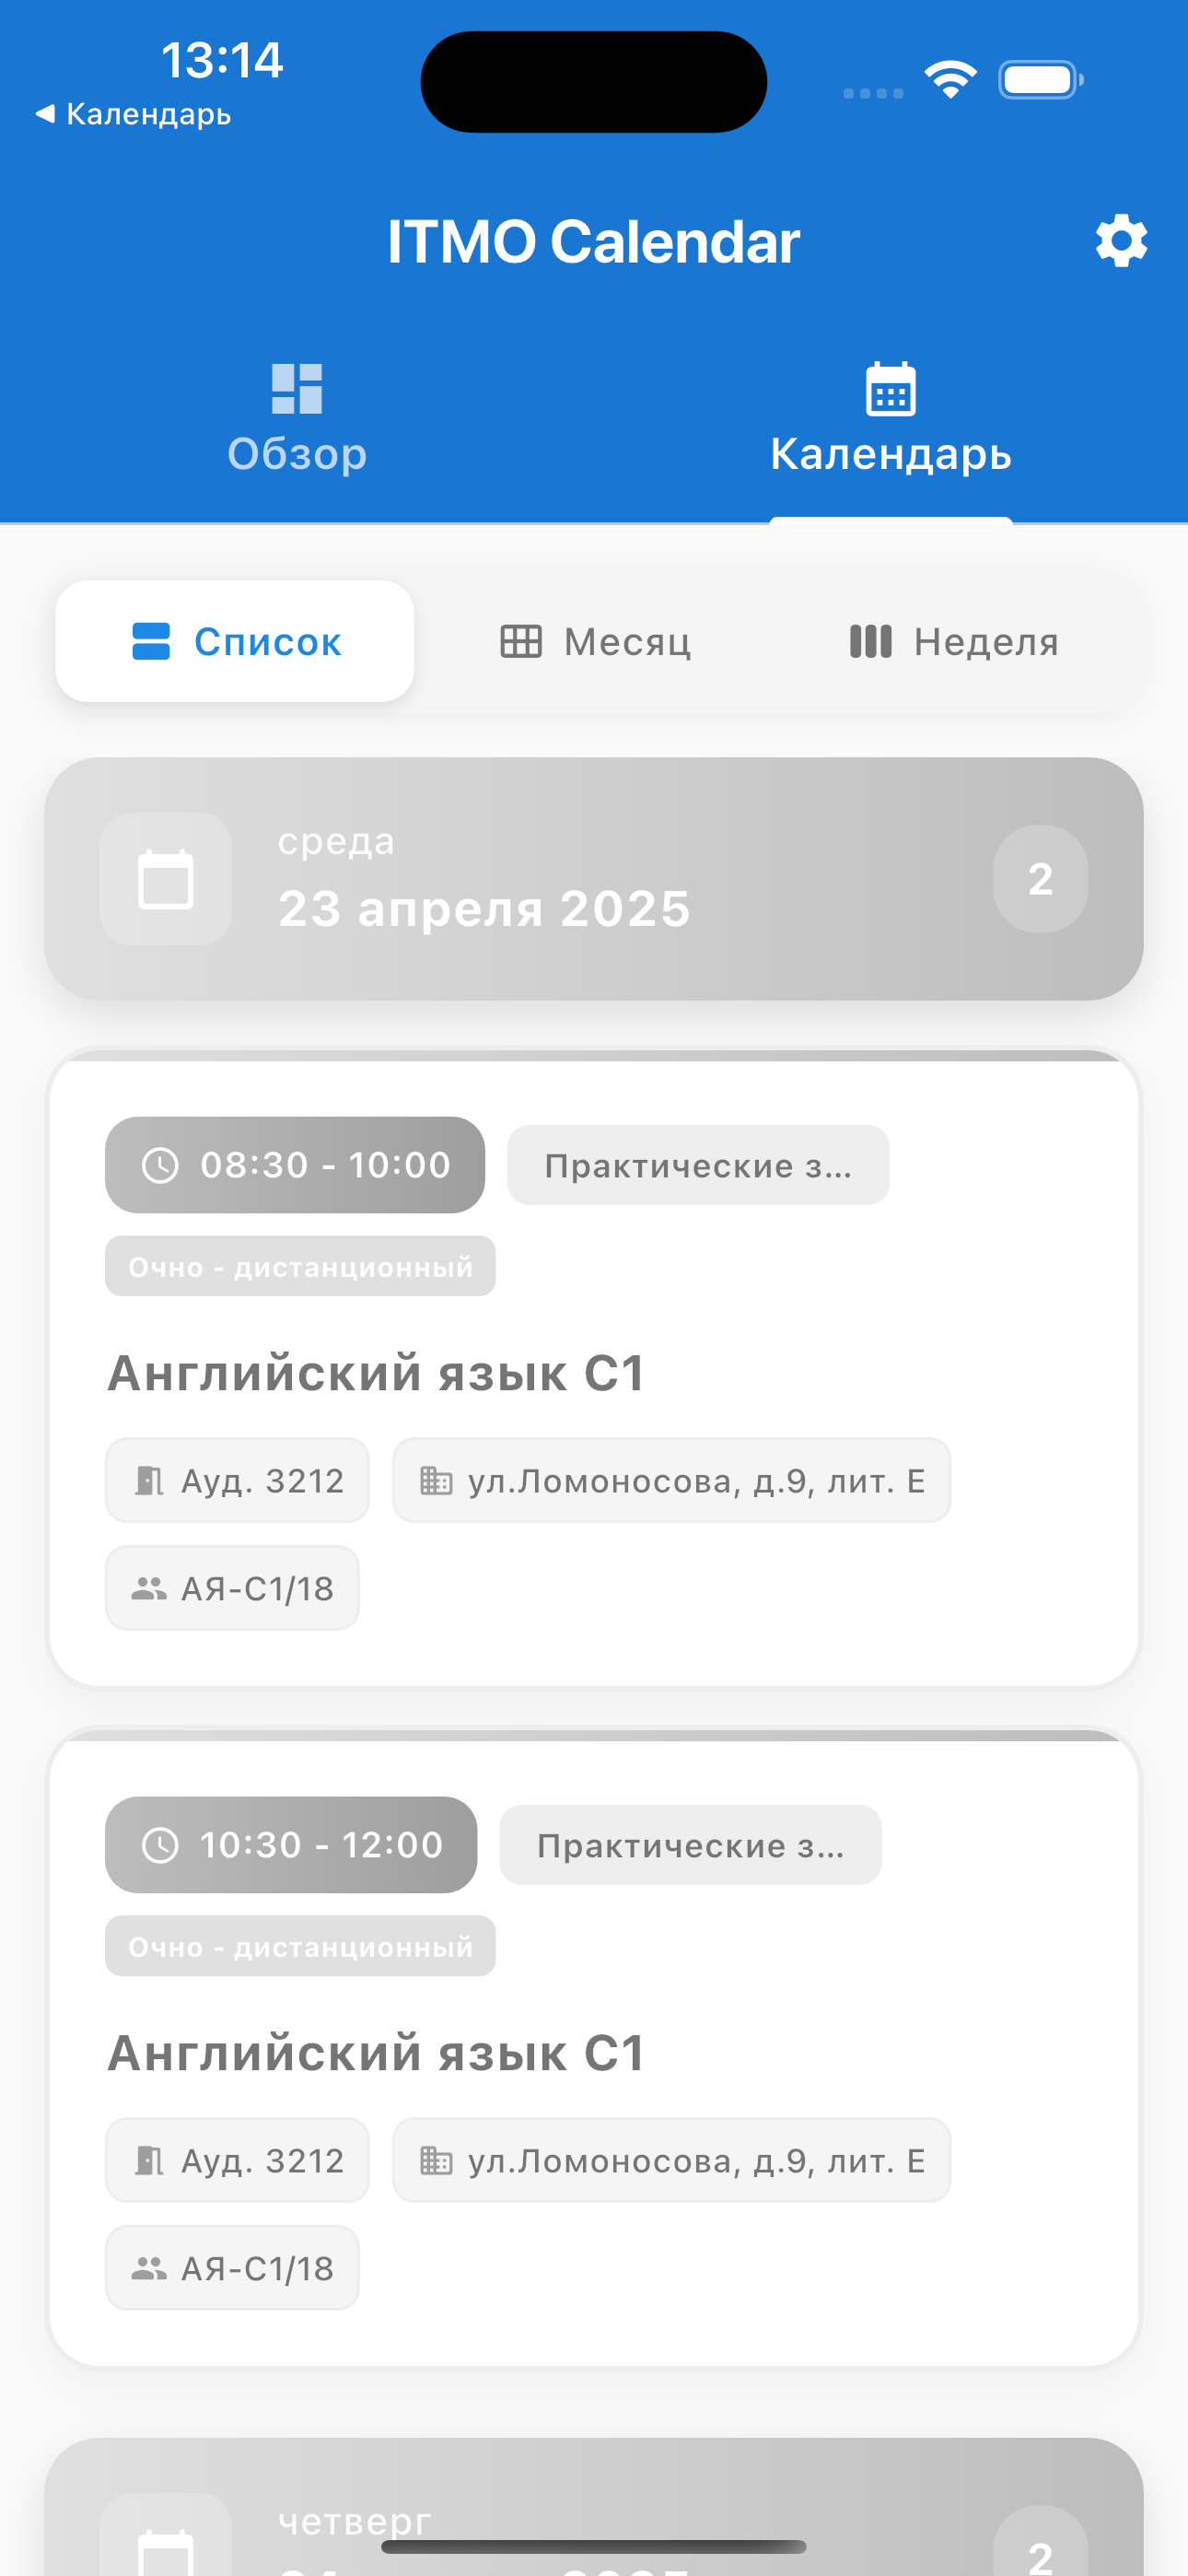
\includegraphics[width=0.6\textwidth]{images/calendar-list.png}
    \caption{Список событий}
    \label{fig:calendar-list}
\end{figure}

\begin{figure}[h!]
    \centering
    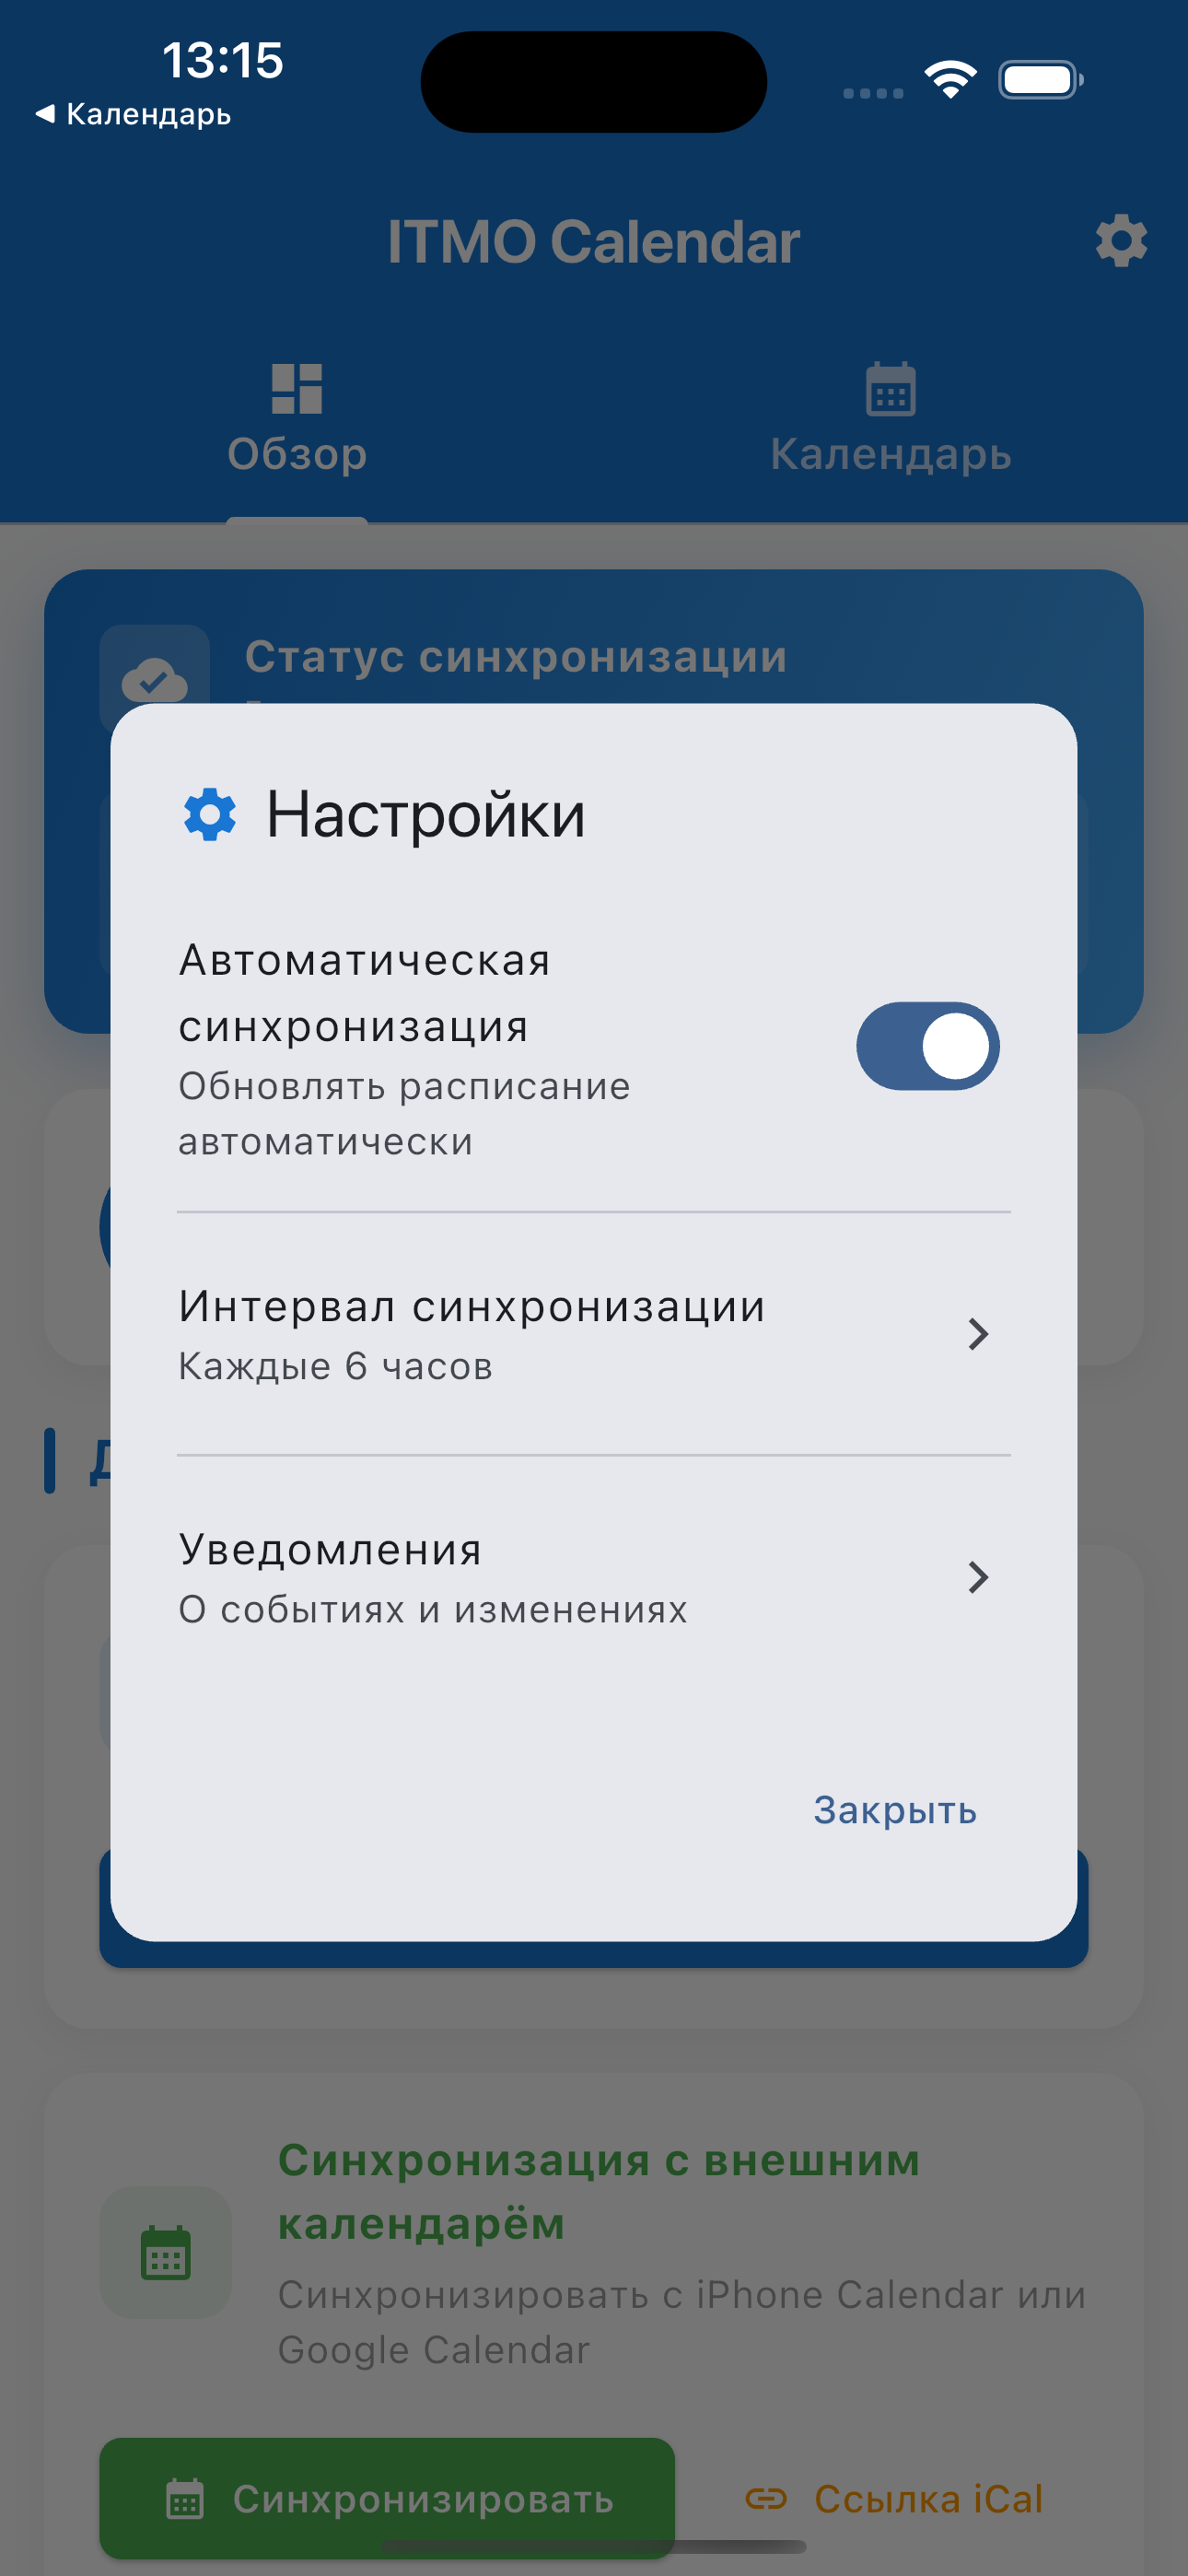
\includegraphics[width=0.6\textwidth]{images/settings.png}
    \caption{Экран настроек}
    \label{fig:settings}
\end{figure}

\begin{figure}[h!]
    \centering
    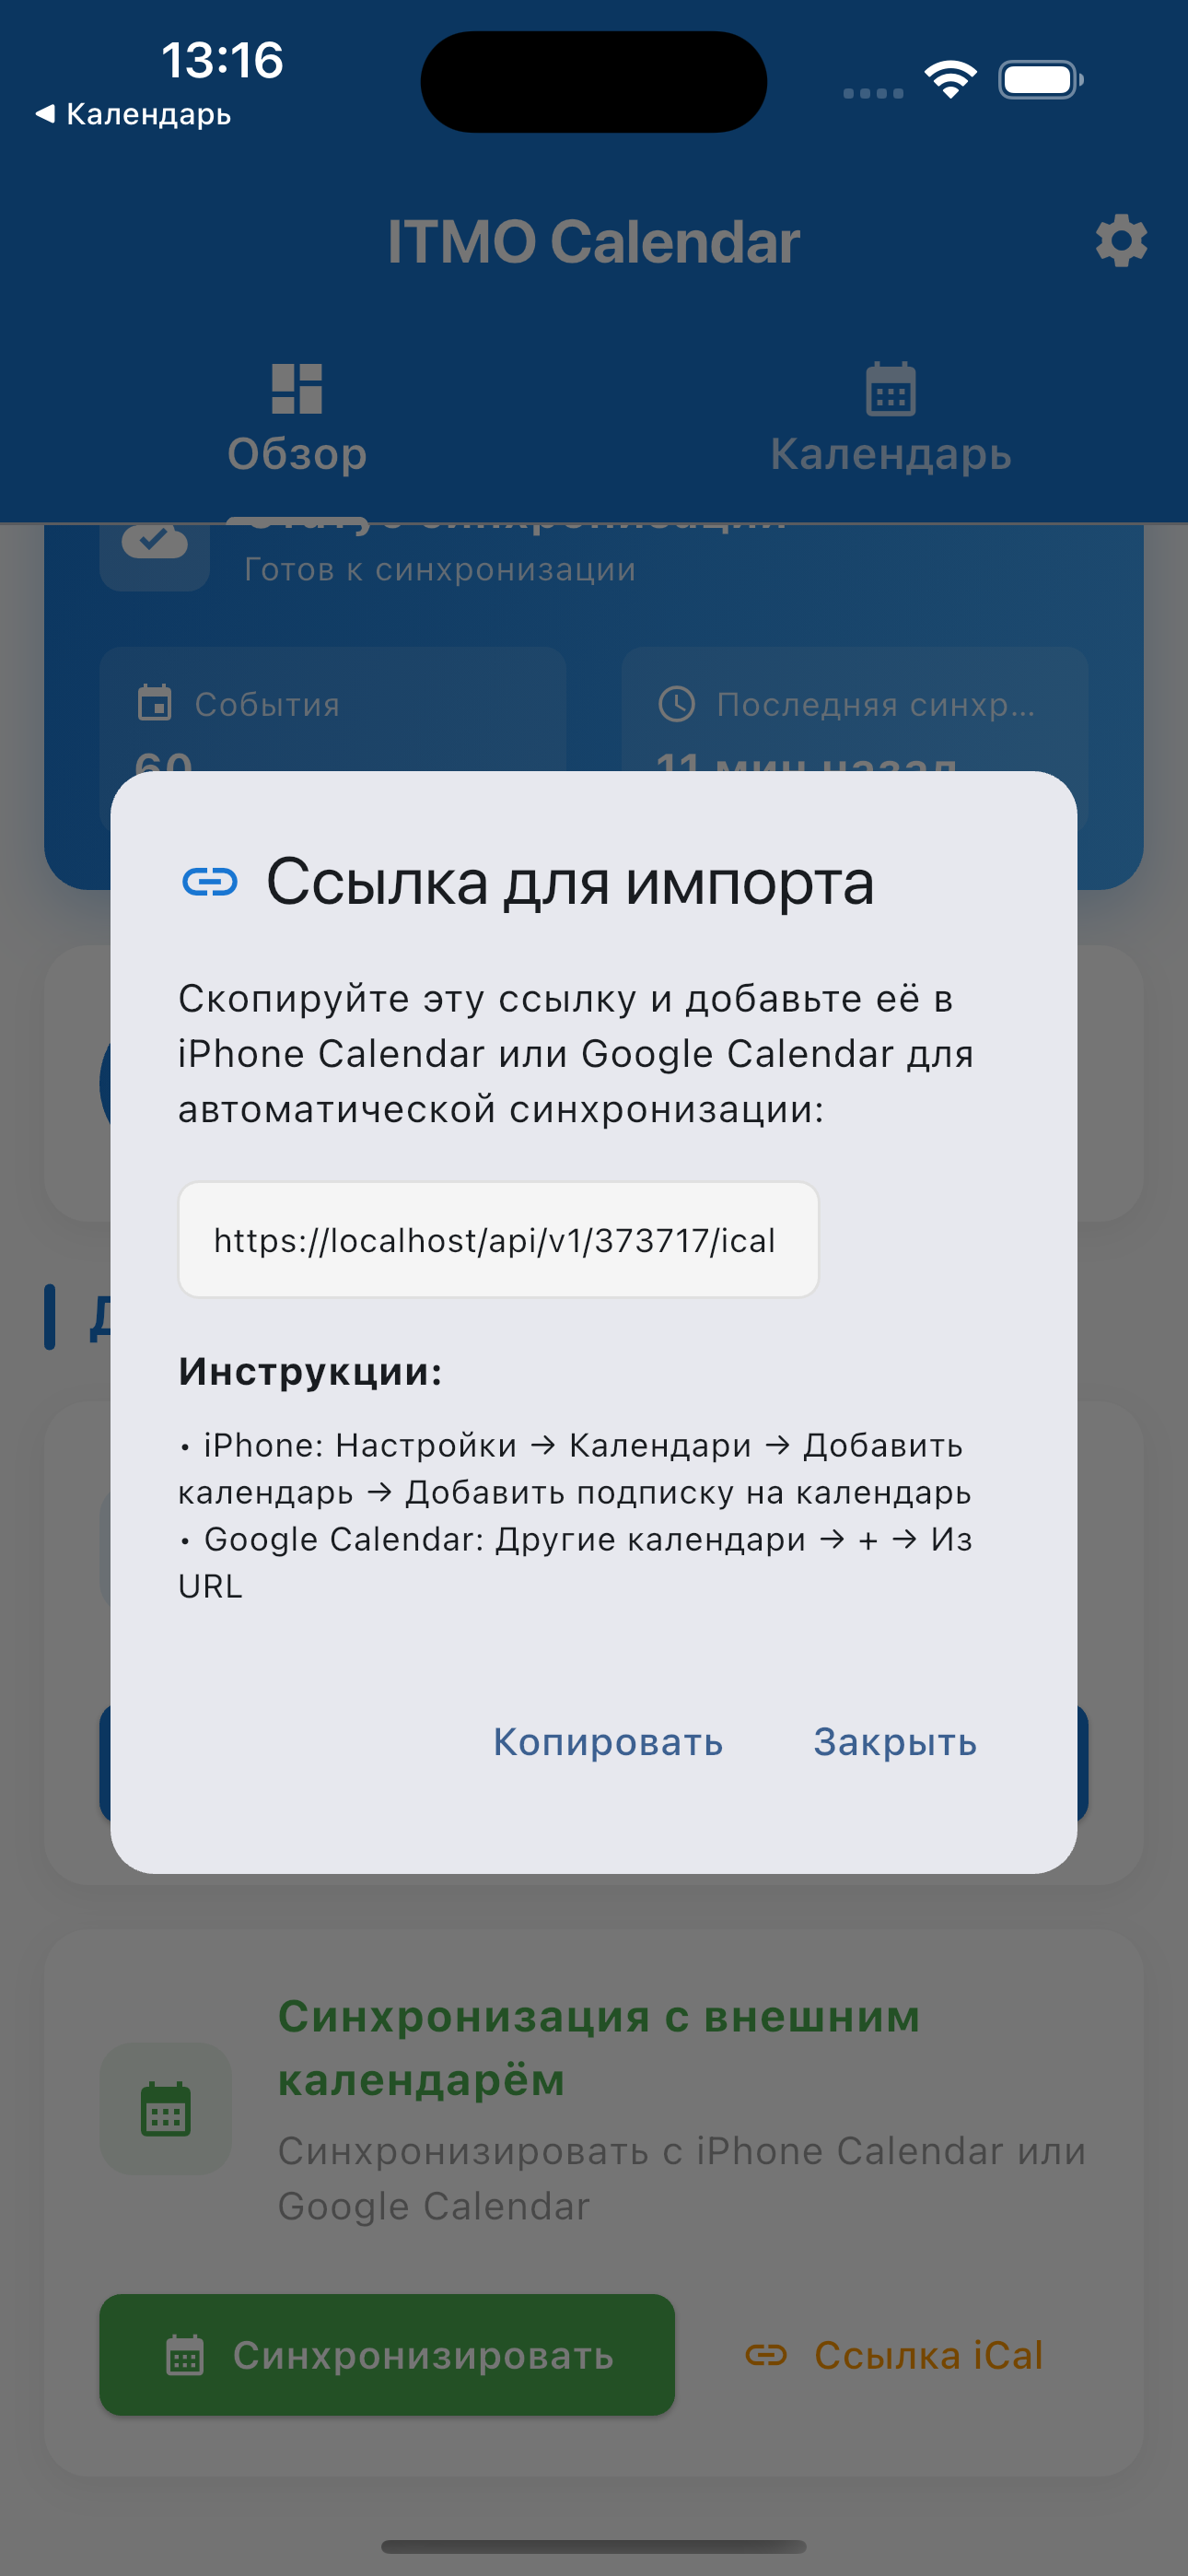
\includegraphics[width=0.6\textwidth]{images/link-for-import-with-instruction.png}
    \caption{Инструкция по импорту календаря}
    \label{fig:import-link}
\end{figure}

\begin{figure}[h!]
    \centering
    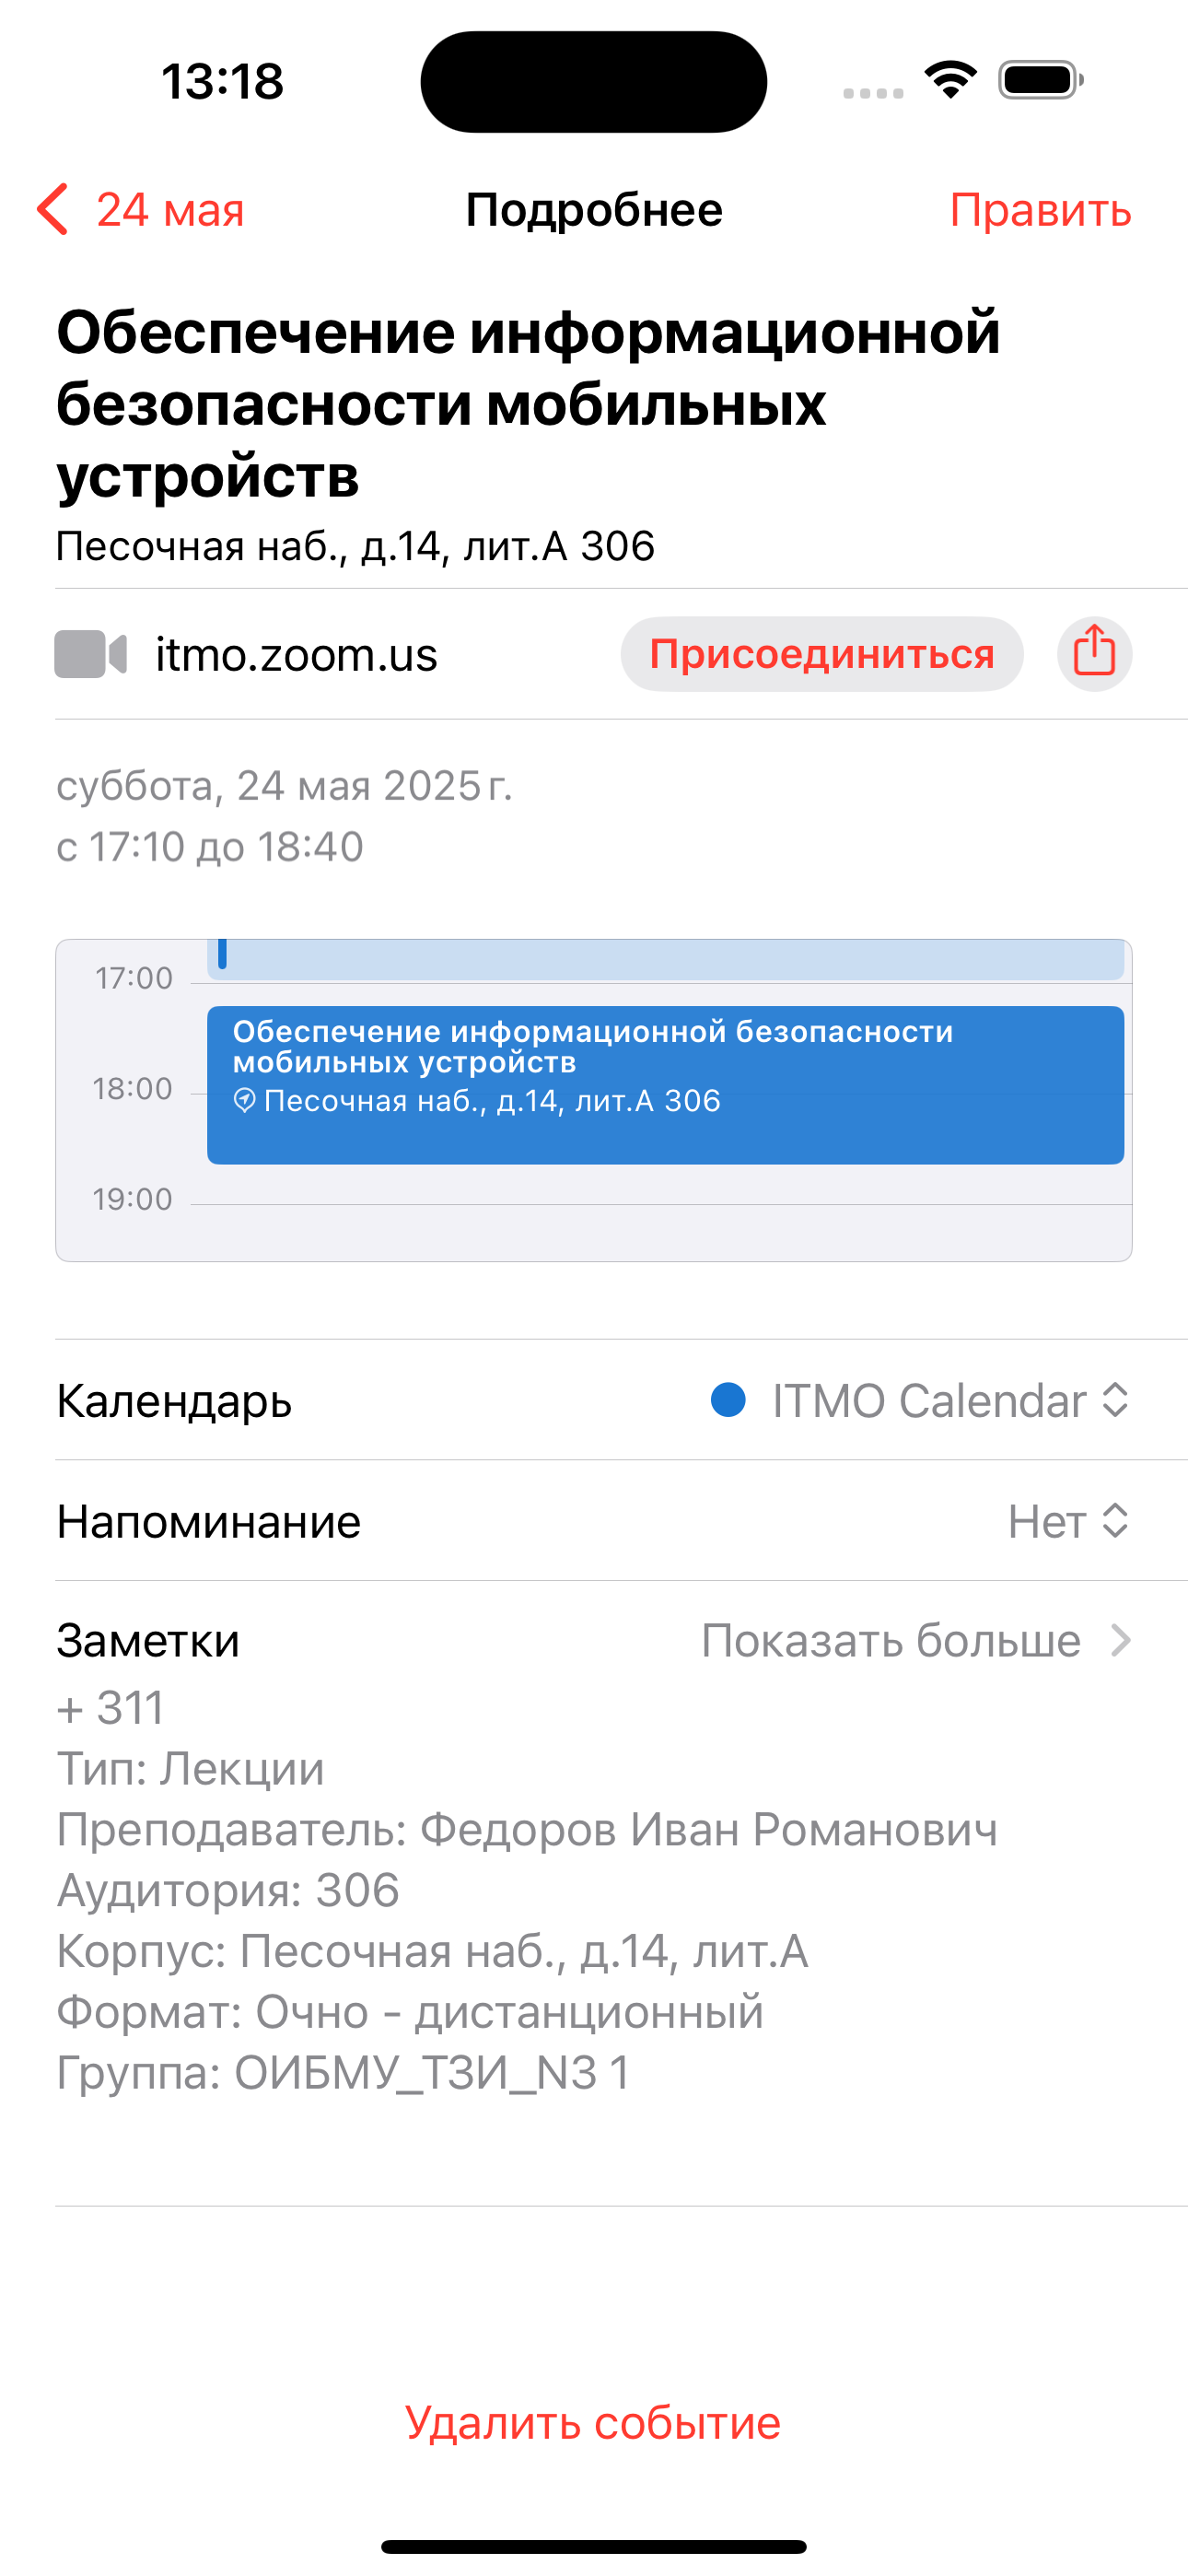
\includegraphics[width=0.6\textwidth]{images/apple-calendar-synced.png}
    \caption{Пример синхронизации с Apple Calendar}
    \label{fig:apple-calendar}
\end{figure}
